\documentclass{SBCbookchapter}
\def\chaptername{Capítulo}
\setcounter{chapter}{8}
\usepackage[T1]{fontenc}
\usepackage{textcomp}
\usepackage[utf8]{inputenc}
\usepackage[english,brazilian]{babel}
\usepackage[protrusion=true,expansion]{microtype}
\usepackage{hyperref}
\hypersetup{colorlinks=true,allcolors=black}
\usepackage{amsmath}
\usepackage{mathtools}
\usepackage{float}
\usepackage{subfigure}
\usepackage{booktabs}
\usepackage{multicol}
\usepackage{multirow}
\usepackage{natbib}
\usepackage{paralist}
\usepackage{xargs}
\usepackage[prependcaption,textsize=tiny,textwidth=2.5cm]{todonotes}
\usepackage{color}
\usepackage{soulutf8}
\setlength{\bibsep}{0.0pt}
%% -------------------------------------------------------------------------
\usepackage{tikz}
\usetikzlibrary{arrows,calc,positioning,shapes,trees}
\newdimen\hdim                  % element height
\newdimen\wdim                  % element width
\newdimen\odim                  % offset distance
\hdim=2.25em
\wdim=2.36\hdim
\odim=\hdim
\tikzstyle{element}=[
  draw=black!60,
  font={\scriptsize\sffamily},
  inner sep=0pt,
  minimum height=\hdim,
  minimum width=\wdim,
  outer sep=0pt,
  rectangle,
  rounded corners=\wdim/10,
  text centered,
  thick,
  top color=white,
  bottom color=black!20,
]
\tikzstyle{arrow}=[
  color=black!60,
  draw=black!60,
  thick,
]
\tikzstyle{arrowlabel}=[
  color=black!60,
  font={\tiny\sffamily\bfseries},
]
\tikzstyle{bin}=[
  dashed,
  draw=black!60,
  font={\tiny\sffamily\bfseries},
  rounded corners=\wdim/12,
]
\tikzstyle{binlabel}=[
  anchor=west,
  color=black!60,
  inner sep=0pt,
  outer sep=0pt,
  pos=0,
  xshift=.25em,
  yshift=-.45em,
]
\tikzstyle{state}=[
  circle,
  draw,
  font={\scriptsize\sffamily},
  inner sep=0pt,
  minimum height=1.5\hdim,
  minimum width=1.5\hdim,
  text width=\hdim,
  outer sep=0pt,
  text centered,
]
\tikzset{
  node distance=\wdim+\odim,
  >=stealth,
  shorten >=.5pt,
}
%% -------------------------------------------------------------------------
\usepackage{listings}
\lstset{%
  basicstyle=\small\ttfamily,
  columns=fullflexible,
  keepspaces=true,
  keywordstyle=\ttfamily,
  language=C,
  escapechar={@},
  mathescape=true,
  showstringspaces=false,
  texcl=true,
  upquote=true,
  extendedchars=true,
  literate=%
    {á}{{\'a}}1%
    {é}{{\'e}}1%
    {í}{{\'i}}1%
    {ó}{{\'o}}1%
    {ú}{{\'u}}1%
    {â}{{\^a}}1%
    {ê}{{\^e}}1%
    {ô}{{\^o}}1%
    {ã}{{\~a}}1%
    {õ}{{\~o}}1%
    {ç}{{\c{c}}}1%
    {€}{\euro}1%
    {§}{\S}1%
    {°}{\textdegree{}}1%
    {ß}{{\ss}}1%
    {Ä}{{\"A}}1%
    {Ö}{{\"O}}1%
    {Ü}{{\"U}}1%
    {µ}{\textmu}1%
    {¹}{{\textsuperscript{1}}}1%
    {²}{{\textsuperscript{2}}}1%
    {³}{{\textsuperscript{3}}}1%
    {¼}{\textonequarter}1%
    {½}{\textonehalf}1%
    {¢}{\textcent}1%
    {“}{``}1%
    {”}{''}1%
    {‘}{`}1%
    {’}{'}1%
    {←}{$\leftarrow$}1%
    {→}{$\rightarrow$}1%
}
\renewcommand{\lstlistingname}{Listagem}
\newdimen\xdim
\xdim=-.5\baselineskip
\lstdefinestyle{command}{
  basicstyle=\small\ttfamily,
  aboveskip=\abovedisplayskip,
  belowskip=.5\belowdisplayskip,
}
\lstdefinestyle{display}{
  aboveskip=\abovedisplayskip,
  basicstyle=\scriptsize\ttfamily,
  belowskip=0pt,
  captionpos=b,
  frame=tb,
  numbers=left,
  numberstyle={\tiny\sffamily},
}
%% -------------------------------------------------------------------------
\def\en#1{\foreignlanguage{english}{\emph{#1}}}
\let\C\lstinline
\def\<#1>{\ensuremath{\left<#1\right>}}

\newcommandx{\rg}[1]{\todo[linecolor=cyan,backgroundcolor=cyan!25,bordercolor=cyan]{#1}}
\newcommandx{\rghl}[2]{{\sethlcolor{cyan}\hl{#1}}\todo[linecolor=cyan,backgroundcolor=cyan!25,bordercolor=cyan]{#2}}


\title{Programando aplicações multimídia no GStreamer}
\author{%
  Guilherme F\null.~Lima,
  Rodrigo C\null.\,M.~Santos,
  Roberto G\null.\,~de~A.~Azevedo
}
\begin{document}
\maketitle
\vskip-1.525\baselineskip\strut
\begin{abstract}
  \begin{otherlanguage}{english}
  This short course is an introduction to GStreamer, one of the main
  free/open-source frameworks for multimedia processing.  We start
  presenting GStreamer, its architecture and the dataflow programming
  model, and then adopt a hands-on approach.  Starting with an example, a
  simple video player, we introduce each concept of GStreamer’s basic C
  API and implement it over the initial example incrementally, so that at
  the end of the course we get a complete video player with support for
  the usual playback operations (start, stop, pause, seek, fast-forward,
  and rewind).  We also discuss sample filters---processing elements that
  manipulate audio and video samples.  We present the various filters
  natively available in GStreamer and show how one can extend the
  framework by creating a plugin with a custom filter that manipulates
  video samples.  The only prerequisite for the short course is a basic
  knowledge of the C programming language.  At the end of the short
  course, we expect that participants acquire a general view of GStreamer,
  and be able to create simple multimedia applications and explore its
  more advanced features.
\end{otherlanguage}

\end{abstract}
\begin{resumo}
  Este minicurso é uma introdução ao GStreamer, um dos principais
  \en{frameworks} de código livre/aberto para processamento de dados
  multimídia.  Começamos apresentando o GStreamer, sua arquitetura e modelo
  de programação baseado em \en{dataflow}, e em seguida, adotamos uma
  abordagem prática.  Partindo de um exemplo inicial, um \en{player} de
  vídeo, introduzimos cada conceito da API~C básica do GStreamer e o
  implementamos sobre o exemplo, incrementando-o, de forma que ao final do
  minicurso obtemos um \en{player} de vídeo completo, com suporte às
  operações usuais de reprodução de vídeo (\en{start}, \en{stop}, \en{seek},
  \en{fast-forward} e~\en{rewind}).  Discutimos também filtros---elementos
  que manipulam amostras de áudio e vídeo---e apresentamos os diversos
  filtros disponíveis nativamente no GStreamer.  Além disso, mostramos como
  estender o \en{framework} criando um \en{plugin} com um filtro simples que
  manipula amostras de vídeo.  O único pré-requisito para o minicurso é um
  conhecimento básico da linguagem de programação~C\null.  Ao final do
  minicurso, esperamos que os participantes tenham uma visão geral do
  GStreamer, e estejam aptos a criar aplicações simples e explorar os
  recursos mais avançados do \en{framework}.
\end{resumo}


\section{Introdução}
\label{sec:intro}

O GStreamer~\cite{gstreamer} é um dos principais \en{frameworks} de código
livre/aberto para processamento de dados multimídia.  Além de robusto e
flexível, ele suporta diversos formatos de áudio e vídeo, e é amplamente
utilizado na indústria e na academia~\cite{gstreamer-apps}.
O \en{framework} em si consiste de um conjunto de bibliotecas~C e
ferramentas relacionadas.  Neste minicurso, apresentamos tanto a parte
conceitual quanto a prática do GStreamer.

Na parte conceitual, discutimos o modelo de computação \en{dataflow} no qual
o GStreamer se baseia, e que também é adotado por outros \en{frameworks} e
linguagens multimídia, por exemplo, DirectShow~\cite{Chatterjee-A-1997},
Pure Data~\cite{Puckette-M-S-2007}, CLAM~\cite{Amatriain-X-2008},
ChucK~\cite{Wang-G-2003}, Faust~\cite{Orlarey-Y-2009}, etc.  Nesse modelo,
uma aplicação multimídia estrutura-se como um grafo em que os nós são
elementos processadores e as arestas representam conexões entre elementos
por onde fluem amostras de áudio e vídeo e dados de controle.  O modelo de
\en{dataflow} é particularmente interessante para multimídia porque
possibilita implementações naturalmente paralelas, modulares e escaláveis.

Na parte prática, apresentamos os principais conceitos da
API~C~\cite{Kernighan-B-W-1988} básica (de baixo nível) do GStreamer~1.8,
sua versão estável mais atual, e ilustramos o uso dessa API a partir da
construção de um reprodutor (\en{player}) de vídeo.  Apesar de aqui estarmos
interessados apenas na reprodução (decodificação e apresentação) de fluxos
de mídia, essa mesma API pode ser utilizada para capturar fluxos de áudio e
vídeo, codificá-los e transmiti-los na rede.  O GStreamer possui uma grande
variedade de componentes para tratar cada uma dessas fases de processamento
e, portanto, pode ser usado para construir diversos tipos de aplicações
multimídia tais como editores de vídeo, transcodificadores, transmissores de
fluxos de mídia, \en{players} de mídia e motores de renderização de
linguagens multimídia.

O restante do capítulo está organizado da seguinte forma.  Na
Seção~\ref{sec:hello} apresentamos uma versão preliminar do exemplo base do
minicurso: um \en{player} de vídeo simples, porém funcional.  Na
Seção~\ref{sec:dissec} discutimos o que está por trás do código
aparentemente simples do exemplo anterior e reconstruímos o mesmo exemplo
usando a API básica do GStreamer; essa versão reconstruída é o ponto de
partida dos incrementos posteriores.  Na Seção~\ref{sec:filtros}
apresentamos alguns do principais filtros de áudio e vídeo disponíveis no
GStreamer e discutimos como integrá-los ao exemplo.  Na Seção~\ref{sec:ops}
adicionamos ao exemplo suporte às operações usuais de controle de reprodução
(\en{start}, \en{stop}, \en{pause}, \en{seek}, \en{fast-foward}
e~\en{rewind}).  Na Seção~\ref{sec:plugins} apresentamos a arquitetura de
\en{plugins} do GStreamer e mostramos como implementar e integrar ao exemplo
um \en{plugin} simples contendo um elemento que manipula amostras de vídeo.
Finalmente, na Seção~\ref{sec:conclusao} discutimos funcionalidades
avançadas do \en{framework} e listamos algumas referências para estudos
posteriores.

Antes de escrever nossa primeira aplicação GStreamer, porém, é preciso
entender o modelo de computação \en{dataflow}, no qual o \en{framework} se
baseia.  No restante desta seção apresentamos esse modelo e discutimos como
ele é instanciado no GStreamer.


\clearpage
\subsection*{O modelo \en{dataflow} e sua instanciação no GStreamer}

No modelo de computação \en{dataflow} os dados são processados enquanto
``fluem'' através de uma rede.  Essa rede estrutura-se como um grafo
dirigido em que os nós representam elementos de processamento, ou atores, e
as arestas representam conexões unidirecionais por onde fluem os dados.  Os
atores recebem dados através de suas portas de entrada e emitem dados
através de suas porta de saída.  Um \en{pipeline} é um \en{dataflow} em que
os dados fluem através das arestas na mesma ordem em que foram
produzidos~\cite{Kahn-G-1977,Lee-E-A-1995}.  O modelo de computação
\en{dataflow}, e em especial o modelo de \en{pipeline}, é interessante para
multimídia porque aproxima a estrutura real do sistema da sua descrição
abstrata, idealizada na forma de diagrama de blocos~\cite{Yviquel-H-2014}.
Além disso, o modelo de \en{dataflow} induz implementações flexíveis e
eficientes já que ele é naturalmente paralelo, modular e escalável:
(1)~paralelo porque conceitualmente os atores executam independentemente uns
dos outros; (2)~modular porque a lógica de processamento está encapsulada
nos atores e pode ser reusada em diversos pontos do \en{dataflow};
e~(3)~escalável porque a estrutura é naturalmente composicional (um
\en{dataflow} pode ser visto como um ator e vice versa).

A Figura~\ref{fig:pipe-tipico} apresenta o leiaute de um \en{pipeline}
típico para processamento multimídia.  O leiaute nesse caso é uma versão
simplificada do \en{pipeline} de uma aplicação GStreamer que reproduz um
vídeo Ogg~\cite{ogg-rfc-3533} .  Os nós da figura representam atores e as
arestas representam as conexões por onde fluem as amostras de áudio e vídeo
e dados de controle.  Na terminologia do GStreamer os atores são chamados de
``elementos'' e as portas de~``\en{pads}''.  Há dois tipos de \en{pads}:
\en{sink pads} e \en{source pads}.  As \en{sink pads} são as portas de
entrada através das quais o elemento consome dados, e as \en{source pads}
são as portas de saída através das quais o elemento produz dados.  Os
elementos são classificados de acordo com o tipo de suas \en{pads}.
Elementos produtores (\en{sources}) possuem apenas \en{source pads}.
Elementos processadores possuem ambos os tipos, \en{source pads} e \en{sink
  pads}.  E, elementos consumidores (\en{sinks}) possuem apenas \en{sink
  pads}.  Consequentemente, produtores apenas produzem dados, processadores
consomem e produzem dados, e consumidores apenas consomem dados.

\begin{figure}[H]
  \centering
  \begin{tikzpicture}
    \node (filesrc) [element] {filesrc};
    \coordinate [above=.5\hdim of filesrc] (A);
    \coordinate [below=.5\hdim of filesrc] (B);
    %%
    \node (oggdemux) [element, right of=filesrc] {oggdemux};
    \coordinate [right of=oggdemux] (C);
    %%
    \node (vorbisdec) [element] at (C|-A) {vorbisdec};
    \node (alsasink) [element, right of=vorbisdec] {alsasink};
    \node (theoradec) [element] at (C|-B) {theoradec};
    \node (xvimagesink) [element, right of=theoradec] {xvimagesink};
    %%
    \draw [->, arrow] (filesrc) -- (oggdemux);
    \coordinate (X) at ($(oggdemux.east)+(0,.25\hdim)$);
    \coordinate (Y) at ($(oggdemux.east)+(0,-.25\hdim)$);
    \draw [->, arrow] (X) -- node [arrowlabel, above] {A} ++(\odim/3,0)
                          -- ($(vorbisdec.west)-(\odim/3,0)$)
                          -- (vorbisdec.west);
    \draw [->, arrow] (Y) -- node [arrowlabel, below] {V} ++(\odim/3,0)
                          -- ($(theoradec.west)-(\odim/3,0)$)
                          -- (theoradec.west);
    \draw [->, arrow] (vorbisdec) -- (alsasink);
    \draw [->, arrow] (theoradec) -- (xvimagesink);
  \end{tikzpicture}
  \caption{Um \en{pipeline} GStreamer que reproduz um arquivo de vídeo Ogg.}
  \label{fig:pipe-tipico}
\end{figure}

Na Figura~\ref{fig:pipe-tipico} há um elemento produtor (``filesrc''), três
processadores (``oggdemux'', ``vorbisdec'' e ``theoradec'') e dois
consumidores (``alsasink'' e ``xvimagesink'').  O elemento ``filesrc''
possui uma única \en{source pad} que está conectada à \en{sink pad} do
elemento subsequente, ``oggdemux''.  Ou seja, os dados produzidos pelo
elemento ``filesrc'' fluem através da sua \en{source pad} para a \en{sink
  pad} do elemento ``oggdemux''.  No diagrama, essa conexão entre as
\en{pads} é representada pela aresta entre os elementos ``filesrc'' e
``oggdemux''.  Similarmente, as demais arestas denotam conexões entre
\en{source pads} e \en{sink pads}.

O processo de desenvolvimento de uma aplicação GStreamer com \en{pipeline}
estático (cuja topologia não muda em tempo de execução) é relativamente
simples.  Basta instanciar os elementos necessários, interconectar suas
\en{pads} e iniciar o \en{pipeline} resultante.  O \en{pipeline} da
Figura~\ref{fig:pipe-tipico}, por exemplo, após iniciado opera da seguinte
forma.
\begin{enumerate}
\item O elemento ``filesrc'' lê um arquivo Ogg armazenado no sistema de
  arquivos e escreve o fluxo de bytes resultante na sua \en{source pad}.
  Ogg é~\cite{ogg-rfc-3533} um formato para multiplexação de fluxos de
  áudio, vídeo e texto.  Vamos assumir que o arquivo Ogg nesse caso contém
  apenas dois fluxos multiplexados: um fluxo de áudio (sequência de amostras
  de áudio) codificado no formato Vorbis~\cite{vorbis}; e um fluxo de vídeo
  (sequência de quadros de imagem) codificado no formato
  Theora~\cite{theora}.
\item O elemento ``oggdemux'' lê da sua \en{sink pad} um fluxo de bytes
  codificado no formato Ogg, demultiplexa-o e escreve os fluxos Vorbis
  (áudio) e Theora (vídeo) resultantes nas \en{source pads} correspondentes.
  Na figura~\ref{fig:pipe-tipico}, a \en{source pad} que recebe o fluxo
  de áudio codificado possui o rótulo~``A'' e a \en{source pad} que recebe o
  fluxo de vídeo codificado possui o rótulo~``V''.
\item O elemento ``vorbisdec'' lê da sua \en{sink pad} um fluxo de bytes
  codificado no formato Vorbis, decodifica-o e escreve o fluxo de áudio~PCM
  resultante na sua \en{source pad}.  Um fluxo de áudio PCM é o que chamamos
  de ``áudio descomprimido'' (\en{raw}), ou seja, é uma sequência de
  amostras obtidas via \en{pulse-code modulation} que representa
  digitalmente o sinal analógico original.
\item O elemento ``theoradec'' opera de maneira análoga.  Ele lê da sua
  \en{sink pad} um fluxo de bytes codificado no formato Theora, decodifica-o
  e escreve o fluxo de vídeo descomprimido (\en{raw}) resultante na sua
  \en{source pad}.  Um fluxo de vídeo descomprimido é uma sequência de
  amostras (quadros) de vídeo em que cada quadro é uma matriz de \en{pixels}
  codificados em algum modelo de cor.  No modelo de cor RGB
  (\en{red-green-blue}), por exemplo, cada \en{pixel} é codificado como uma
  sequência de três inteiros que representam tonalidades de vermelho, verde
  e azul.
\item O elemento ``alsasink'' lê um fluxo de áudio descomprimido da sua
  \en{sink pad} e utiliza a biblioteca ALSA~\cite{alsa} para reproduzir as
  amostras do fluxo nos alto-falantes.
\item O elemento ``xvimagesink'' lê um fluxo de vídeo descomprimido da sua
  \en{sink pad} e utiliza a biblioteca X11~\cite{x11} para reproduzir os
  quadros do fluxo na tela.
\end{enumerate}

A função de um \en{pipeline}, isto é, o que ele faz ou computa, é o
resultado da combinação da função dos seus elementos que, conceitualmente,
operam em paralelo.  O \en{pipeline} anterior, portanto, (1)~lê um arquivo
Ogg, (2)~demultiplexa-o, (3--4)~decodifica os fluxos de áudio e vídeo
resultantes e~(5--6) reproduz os fluxos decodificados nos dispositivos de
saída correspondentes (alto-falantes e tela).  Conceitualmente, tudo isso
acontece em paralelo, ou seja, podemos assumir que enquanto os \en{sinks}
``alsasink'' e ``xvimagesink'' estão exibindo amostras, o \en{source}
``filesrc'' está lendo bytes do disco, o demultiplexador ``oggdemux'' está
demultiplexando dados Ogg e os decodificadores ``vorbisdec'' e ``theoradec''
estão decodificando dados Vorbis e Theora.

A descrição anterior seria suficiente se estivéssemos interessados apenas em
exibir as amostras decodificadas o mais rápido possível.  Mas esse não é
caso.  Queremos ``tocar'' o vídeo original em tempo real, isto é,
reproduzi-lo nas mesmas condições em que ele foi gravado (amostrado).  Sendo
assim, para que o vídeo seja reproduzido corretamente, suas amostras de áudio
e vídeo devem ser exibidas na taxa correta.  Valores típicos para essas
taxas são~44100Hz para amostras de áudio e~30Hz para amostras de vídeo; ou
seja, a cada~22{,}67\textmu{s} uma nova amostra de áudio deve ser enviada ao
dispositivo de saída de áudio, e a cada~33{,}33ms uma nova amostra de vídeo
deve ser enviada ao dispositivo de saída de~vídeo.

No GStreamer, em geral, são os elementos \en{sink} os responsáveis por
controlar as taxas de exibição de amostras.  Por exemplo, no \en{pipeline} da
Figura~\ref{fig:pipe-tipico}, para manter a taxa de reprodução necessária, os
\en{sinks} ``alsasink'' e ``xvimagesink'' armazenam as amostras recebidas numa
fila interna e exibem-nas (consomem-nas) apenas no momento adequado.  Já os
outros elementos operam livres---consomem e produzem dados em taxas
arbitrárias.  Se durante a execução os elementos que precedem os \en{sinks}
operarem rápido o bastante, as filas dos \en{sinks} nunca ficarão vazias e
todas as amostras serão exibidas no momento correto, mas esse nem sempre é o
caso.

Se os elementos que precedem os \en{sinks} operarem abaixo da taxa de consumo
dos \en{sinks}, pode ser que alguma das filas internas fique vazia e,
caso chegue o momento de exibir uma amostra, o \en{sink} simplesmente não tenha
o que exibir, causando interrupções ou saltos na reprodução (amostras
``atrasadas'' quando chegarem serão descartadas).  Há ainda o problema inverso.
Se os elementos que precedem os \en{sink} operarem muito acima da taxa de
consumo dos \en{sinks}, pode ser que a capacidade da fila interna seja excedida
e amostras sejam~perdidas.  Para evitar ambos os problemas, esvaziamento ou
estouro das filas, ou mesmo para limitar o uso de CPU, os \en{sinks}
normalmente enviam eventos de QoS (\en{quality of service}) para os elementos
que os precedem, que indicam o quão atrasada ou adiantada está cada amostra que
chega.  Assim, os elementos anteriores (produtores e processadores) podem
capturar esses eventos e usar a informação de retardo para ajustar a sua taxa
de operação.

Dois tipos de dados trafegam através das conexões (arestas) de um
\en{pipeline} GStreamer: segmentos de dados (\en{buffers}) e eventos
(\en{events}).  Os \en{buffers} carregam segmentos do conteúdo processado
entre \en{pads} (por exemplo, amostras de áudio e vídeo codificadas ou
\en{raw}) e fluem exclusivamente na direção das conexões, ou seja, de
\en{source pads} para \en{sink pads}.  Já os eventos carregam informação de
controle; eles também fluem entre conexões, mas podem percorrê-las em ambos
os sentidos: fluxo abaixo (\en{downstream}), de \en{source pads} para
\en{sink pads}, ou fluxo acima (\en{upstream}), de \en{sink pads} para
\en{source pads}.  Além de eventos de QoS, elementos podem emitir eventos de
EOS (\en{end-of-stream}) que indicam o fim do fluxo, eventos de \en{seek}
que indicam deslocamentos no fluxo e eventos de \en{flush} que sinalizam que
\en{caches} internos devem ser descarregados.

\en{Buffers} e eventos percorrem as conexões em paralelo.  Ou seja,
conceitualmente cada conexão entre as \en{pads} dos elementos pode ser
entendida como consistindo de dois canais, um canal unidirecional para
\en{buffers} e outro canal bidirecional para eventos.
A Figura~\ref{fig:conexao} ilustra a estrutura conceitual de uma conexão
entre \en{pads}.  Na figura,``B'' é o canal de \en{buffers} e ``E'' é o
canal de eventos.

\begin{figure}[H]
  \centering
  \begin{tikzpicture}
    \node [cylinder, thick, draw=black!60, cylinder uses custom fill,
           cylinder end fill=black!30, cylinder body fill=black!20,
           minimum height=\wdim, minimum width=\hdim] (c) {};
    \coordinate (x) at ($(c.before top|-c.east)+(0,.15\hdim)$);
    \coordinate (y) at ($(c.before top|-c.east)-(0,.15\hdim)$);
    \coordinate (x0) at ($(c.west|-x)+(.25pt,0)$);
    \coordinate (y0) at ($(c.west|-y)+(.25pt,0)$);
    \draw [->,arrow] (x)
    -- node [arrowlabel, above, pos=.4] {B} ++(\odim,0);
    \draw [arrow] (x0) -- ++(-\odim,0);
    \draw [->,arrow] (y)
    -- node [arrowlabel, below, pos=.4] {E} ++(\odim,0);
    \draw [->,arrow] (y0) -- ++(-\odim,0);
  \end{tikzpicture}
  \caption{Estrutura conceitual de uma conexão entre \en{pads} no
    GStreamer.}
  \label{fig:conexao}
\end{figure}
\vskip-\baselineskip

A discussão do modelo \en{dataflow} e da sua instanciação no GStreamer se
encerra aqui.  Na maior parte do tempo, programar no GStreamer consiste em
montar \en{pipelines} e controlar seu funcionamento.  Até agora discutimos
de maneira abstrata os conceitos envolvidos nessa montagem e controle.  A
partir da próxima seção, veremos como utilizar esses conceitos na prática.


\section{Olá mundo: Tocando um vídeo}
\label{sec:hello}

Nosso objetivo nesta seção é usar o GStreamer para tocar um vídeo.  Para
tal, poderíamos implementar o \en{pipeline} da Figura~\ref{fig:pipe-tipico},
mas há uma maneira mais simples: basta usar o elemento ``playbin''.
A Listagem~\ref{lst:hello} apresenta um programa~C que faz exatamente isso.

\lstinputlisting[
style=display,
caption={Tocando um vídeo no GStreamer usando o elemento ``playbin''.},
label={lst:hello},
]{src/hello.c}

Vejamos o propósito de cada linha da Listagem~\ref{lst:hello}.  A linha~1
inclui as declarações da GLib~\cite{glib}, a biblioteca de portabilidade do
projeto GNOME~\cite{gnome}, e a linha~2 inclui as declarações do
GStreamer---o GStreamer depende do \en{framework} GObject~\cite{gobject} da
GLib para programação orientada a objetos em~C\null.  Na listagem, as
chamadas com prefixo ``\C{g_}'' ou ``\C{G_}'' e referem-se à funções e
macros da GLib, e as chamadas com prefixo ``\C{gst_}'' ou ``\C{GST_}'' e as
declarações com prefixo ``\C{Gst}'' referem-se à funções, macros e tipos do
GStreamer.

A chamada~\C{gst_init}, linha~12, inicializa o GStreamer e trata os
argumentos com prefixo ``-\,-gst-'' em \C{argv}.

A próxima chamada, linha~14, cria um elemento ``playbin'' que é também o
\en{pipeline} da aplicação.  No GStreamer, o \en{pipeline} é, ele próprio,
um elemento---que contém outros elementos mas não possui \en{pads}.  Tais
elementos contêiner são chamados de ``\en{bins}''.  A função
\C{gst_element_factory_make} aloca e retorna um novo elemento
(\C{GstElement}) do tipo especificado.  O primeiro parâmetro da função é o
nome da fábrica do tipo e o segundo parâmetro (opcional) é o nome a ser
atribuído ao elemento retornado.  O nome do elemento pode ser usado depois,
por exemplo, para procurar esse elemento em um \en{pipeline}.  No exemplo da
Listagem~\ref{lst:hello}, a chamada cria e retorna um elemento do tipo
``playbin'' chamado ``hello''.  Um elemento ``playbin'' nada mais é do que
um \en{pipeline} que se autoconfigura.  Dada uma URI, assim que o
``playbin'' é iniciado ele determina o tipo do conteúdo da URI e constrói um
\en{pipeline} apropriado para reproduzi-la.

A chamada \C{g_assert_nonnull}, linha~15, é uma asserção que garante que a
chamada anterior funcionou corretamente, isto é, retornou um elemento válido
(não nulo).

A chamada \C{gst_filename_to_uri}, linha~17, constrói uma URI a partir do
caminho de um arquivo.  Nesse caso, ``bunny.ogg'' é caminho do arquivo de
vídeo Ogg que queremos tocar.  O vídeo em si é o curta de animação ``Big
Buck Bunny''~\cite{bunny} produzido pelo Blender Institute e licenciado via
Creative Commons.

A chamada \C{g_object_set}, linha~19, atribui a URI criada anteriormente à
propriedade ``uri'' do elemento ``playbin''.  Note que \C{g_object_set} é
uma função do GObject.  Todo elemento (\C{GstElement}) é também um objeto
(\C{GObject}), e todo objeto possui propriedades cujos valores podem ser
obtidos via \C{g_object_get} e alterados via \C{g_object_set}.

A chamada \C{g_free}, linha~20, libera a \en{string} alocada na linha~16.
Nesse ponto, a \en{string} já não é mais necessária pois foi copiada pela
chamada \C{g_object_set} anterior.

A chamada \C{gst_element_set_state}, linha~22, inicia o \en{pipeline} da
aplicação, isto é, transiciona o elemento ``playbin'' do seu estado inicial
\en{null} (\C{GST_STATE_NULL}) para o estado \en{playing}
(\C{GST_STATE_PLAYING}).  Na Seção~\ref{sec:dissec}, vamos discutir em
detalhes as consequências internas dessa transição.  Por enquanto, basta
dizer que nesse ponto o elemento ``playbin''~(1) inspeciona o conteúdo
apontado pela URI configurada, (2)~instancia e interconecta os elementos
necessários para reproduzir esse conteúdo, (3)~inicia a sua reprodução numa
\en{thread} separada e~(4) devolve o controle à \en{thread} principal da
aplicação.

A chamada \C{g_assert}, linha~23, é uma asserção que garante que a
requisição de transição de estado anterior foi bem sucedida.  Após essa
linha, podemos assumir que o vídeo está tocando e que aplicação possui pelo
menos duas \en{threads}: a \en{thread} principal, que está prestes a
executar a linha~23, e uma ou mais \en{threads} secundárias, que operam o
\en{pipeline}.  A \en{thread} principal é chamada de ``\en{thread} da
aplicação'' e as \en{threads} secundárias são chamadas de ``\en{streaming
  threads}''.  As \en{streaming threads} se comunicam com a \en{thread} da
aplicação através de mensagens assíncronas postadas em um barramento
(\en{bus}) associado ao \en{pipeline}.  Essas mensagens informam a
\en{thread} da aplicação sobre acontecimentos internos do \en{pipeline}, por
exemplo, mudança de estado de elementos, fim do fluxo, erros, \en{warnings},
etc., e permitem que a aplicação reaja da maneira apropriada.

A chamada \C{gst_element_get_bus}, linha~25, obtém uma referência para o
barramento de mensagens (\en{bus}) do \en{pipeline} do ``playbin''.

A próxima chamada, linha~26, bloqueia a \en{thread} da aplicação até que uma
mensagem de erro ou de EOS (\en{end-of-stream}, ``fim do fluxo'') seja
postada no barramento.  Ou seja, a \en{thread} da aplicação aguarda nessa
chamada até que um erro aconteça ou até que o vídeo seja reproduzido
completamente.  A função \C{gst_bus_timed_pop_filtered} recebe o \en{bus}, o
tempo máximo de espera e a máscara dos tipos das mensagens a serem
aguardadas, e bloqueia até que o tempo máximo seja atingido ou até que uma
mensagem de um dos tipos esperados seja postada no \en{bus}.  A função
retorna \C{NULL} caso o tempo máximo seja atingido ou retorna uma referência
para a mensagem recebida.  Na Listagem~\ref{lst:hello}, estamos aguardando
por um tempo ilimitado (\C{GST_TIME_CLOCK_NONE}) uma mensagem de erro
(\C{GST_MESSAGE_ERROR}) ou uma mensagem de EOS (\C{GST_MESSAGE_EOS}) que
após a chamada é armazenada na variável \C{msg}.

A chamada \C{gst_message_unref}, linha~27, libera a mensagem retornada na
chamada da linha anterior.  Nesse ponto, ou houve um erro ou a reprodução
chegou ao fim.

A chamada \C{gst_object_unref}, linha~28, libera a referência para o
\en{bus} do ``playbin'', obtida na linha~25.  A função \C{gst_object_unref} é
um pseudônimo (\en{alias}) para a função \C{g_object_unref}, que libera uma
referência para um \C{GObject}.  No GStreamer, a maioria dos tipos que são
``objeto'' herdam  de \C{GstObject} que, por sua vez, herda de \C{GObject}.

A chamada \C{gst_element_set_state}, linha~30, para o \en{pipeline} da
aplicação (caso ele ainda não esteja parado) e libera os recursos utilizados
durante o seu processamento, isto é, transiciona o elemento ``playbin'' de
volta para o estado inicial \en{null}.

Finalmente, a chamada \C{gst_object_unref}, linha~31, libera o próprio
elemento ``playbin'', alocado na linha~14.

Se tudo correr bem, ao executar o programa ``Olá mundo'' anterior uma nova
janela aparece na tela e o vídeo é reproduzido do inicio ao fim.
A Figura~\ref{fig:bunny} apresenta um quadro do vídeo em questão.  Para
rodar o exemplo, porém, primeiro é preciso compilá-lo.

\begin{figure}[H]
  \centering
  
\includegraphics[scale=.115]{media/frame}
  \caption{Quadro do vídeo \en{Big Buck Bunny}~\cite{bunny}.}
  \label{fig:bunny}
\end{figure}


\subsection*{Compilando o programa ``Olá mundo'' no GNU/Linux}

Para compilar o programa da Listagem~\ref{lst:hello} precisamos informar ao
compilador~C o caminho do diretório contendo os cabeçalhos da GLib e do
GStreamer.  Além disso, precisamos informar ao \en{linker} o caminho e o
nome das bibliotecas dinâmicas correspondentes.  No GNU/Linux, a maneira
mais fácil de se fazer isso é através da ferramenta \en{pkg-config}.  Por
exemplo:
\begin{lstlisting}[style=command]
@\$@ cc hello.c -o hello `pkg-config --cflags --libs glib-2.0\
        gstreamer-1.0`
\end{lstlisting}

Esse comando compila e \en{link}-edita o programa da
Listagem~\ref{lst:hello} (``hello.c'') e gera um executável chamado
``hello''.  As opções ``-\,-cflags'' e ``-\,-libs'' do comando
\en{pkg-config} instruem-no a emitir as \en{flags} de compilação e
\en{link}-edição apropriadas para os módulos listados, no caso, ``glib-2.0''
e ``gstreamer-1.0''.  Observe que a chamada do comando \en{pkg-config}
aparece entre crases.  Ou seja, antes de avaliar o comando mais externo,
\en{cc}, que é a chamada do compilador~C, o interpretador de comandos
(\en{shell}) executa o comando \en{pkg-config} e substitui o texto entre
crases pelo resultado dessa execução.  Por exemplo, no nosso ambiente, o
comando anterior avalia para:
\begin{lstlisting}[style=command]
@\$@ cc hello.c -o hello\
     -pthread\
     -I/usr/include/gstreamer-1.0\
     -I/usr/lib/gstreamer-1.0/include\
     -I/usr/include/glib-2.0\
     -I/usr/lib/glib-2.0/include\
     -lgstreamer-1.0 -lgobject-2.0 -lglib-2.0
\end{lstlisting}

Uma forma de tornar o processo de compilação menos trabalhoso é escrever um
\en{makefile} com a descrição da sequência de comandos que constrói o
programa.  A Listagem~\ref{lst:makefile} apresenta o \en{makefile} (arquivo
texto chamado ``Makefile'') que usamos para construir os exemplos do
minicurso.  Na listagem, a variável \C{PROGRAMS}, linha~1, contém o nome dos
programas a serem construídos.  A variável \C{MODULES}, linha~2, contém os
nomes dos módulos do \en{pkg-config} necessários.  E as variáveis \C{CFLAGS}
e \C{LDFLAGS}, linhas~3 e~4, contém as \en{flags} de compilação e
\en{link}-edição correspondentes.  O restante do arquivo, linhas~5--8,
define os alvos ``all'' e ``clean''.  (Na linha~7, o primeiro caractere é um
TAB\null.)  Uma vez escrito o \en{makefile}, para construir o programa basta
executar o comando ``\C{make}'' (ou ``\C{make all}'') e para remover os
arquivos gerados pelo compilador basta executar ``\C{make clean}''.
(Veja~\cite{Gough-B-J-2005,Mecklenburg-R-2005} para mais informações sobre
como compilar programas e escrever \en{makefiles} no GNU/Linux.)

\lstinputlisting[
style=display,
mathescape=no,
caption={\en{Makefile} que constrói o programa ``Olá mundo''.},
label={lst:makefile},
]{src/Makefile.hello}


\section{Tocando áudio e vídeo
a partir de elementos básicos}
\label{sec:dissec}

Na Seção~\ref{sec:hello} utilizamos o elemento ``playbin'' para tocar um
vídeo Ogg no GStreamer.  Nesta seção, nosso objetivo é construir a mesma
aplicação, mas dessa vez sem usar o elemento ``playbin''.  Usando apenas
elementos básicos (\en{sources}, demultiplexadores, decodificadores e
\en{sinks}) vamos construir um \en{pipeline} semelhante ao da
Figura~\ref{fig:pipe-tipico}, Seção~\ref{sec:intro}, que lê um arquivo Ogg
do disco, demultiplexa-o, e decodifica e reproduz os fluxos de áudio e vídeo
resultantes.  Antes disso, porém, vejamos um exemplo mais simples.


\subsection*{Tocando um arquivo de áudio MP3}

A Listagem~\ref{lst:mp3} apresenta um programa que reproduz um arquivo de
áudio~MP3~\cite{mp3} do disco.  Para tal, o programa monta um \en{pipeline}
com três elementos: ``filesrc'', ``mad'' e ``alsasink''.  Como vimos, no
GStreamer o próprio \en{pipeline} é um elemento---um elemento sem \en{pads}
que contém outros elementos.  Na listagem, a chamada da linha~15 aloca o
elemento \en{pipeline}, que inicialmente está vazio, e as chamadas das
linhas~16--18, alocam os elementos ``filesrc'', ``mad'' e ``alsasink''.  (As
chamadas anteriores, linhas~11--13, inicializam o GStreamer e testam se o
programa foi chamado corretamente, isto é, se o caminho para o arquivo~MP3
está em \C{argv[1]}.)

\lstinputlisting[
float={h},
style=display,
caption={Tocando um arquivo de áudio MP3.},
label={lst:mp3},
]{src/mp3.c}

Na Seção~\ref{sec:intro}, discutimos a operação dos elementos ``filesrc'' e
``alsasink''.  O primeiro lê um arquivo do disco e gera um fluxo de bytes
correspondente, e o segundo lê um fluxo de amostras de áudio PCM e as
reproduz no dispositivo de saída de áudio.  Aqui a novidade é o elemento
processador, mais precisamente, o decodificador ``mad''.  Ele lê da sua
\en{source pad} um fluxo de bytes no formato~MP3, decodifica-o via
MAD~\cite{mad} (biblioteca para decodificação de áudio MP3) e escreve na sua
\en{sink pad} o fluxo de áudio PCM resultante.  Apesar de os três elementos,
``filesrc'', ``alsasink'' e ``mad'', fazerem parte do GStreamer, na prática,
eles pertencem a pacotes diferentes, distribuídos separadamente.

A distribuição oficial do GStreamer possui cinco pacotes principais:
(1)~\en{gstreamer}, contendo o núcleo do \en{framework};
(2)~\en{gst-plugins-base}, contendo apenas os elementos básicos;
(3)~\en{gst-plugins-good}, contendo elementos cuja implementação é
considerada de boa qualidade e cuja licença é~LGPL (\en{Lesser {GNU} General
  Public License}); (4)~\en{gst-plugins-ugly}, contendo elementos cuja
implementação é também considerada de boa qualidade mas que têm licenças
problemáticas; e (5)~\en{gst-plugins-bad}, contendo elementos de qualidade
inferior.\footnote{Essa terminologia é inspirada clássico de faroeste ``The
  Good, the Bad and the Ugly'' (1966).}  O único pacote absolutamente
necessário é o \en{gstreamer}.  Os demais incrementam-no instalando
bibliotecas e \en{plugins} contendo elementos especializados.  O elemento
``filesrc'', por exemplo, está no \en{plugin} ``coreelements'' do pacote
\en{gstreamer}.  Já o elemento ``alsasink'' está no \en{plugin} ``alsa'' do
pacote \en{gst-plugins-base}, e o elemento ``mad'' está no \en{plugin}
``mad'' do pacote \en{gst-plugins-ugly}.  Você pode descobrir os elementos e
\en{plugins} disponíveis na sua instalação através do comando
``\C{gst-inspect}''---voltaremos a falar desse comando no final da seção.

De volta à Listagem~\ref{lst:mp3}, a chamada \C{g_assert} na linha~19
assegura que as chamadas \C{gst_element_factory_make} anteriores foram bem
sucedidas.  Isto é, testa se os elementos ``pipeline'', ``filesrc'', ``mad''
e ``alsasink'' foram de fato alocados.  Um erro comum é tentar instanciar um
elemento de um \en{plugin} que não está instalado.  Na listagem, se isso
acontecer a chamada \C{gst_element_factory_make} retornará~\C{NULL} e a
asserção falhará, abortando o programa.

Continuando, a chamada da \C{gst_bin_add_many}, linha~21, adiciona três elementos 
ao \en{pipeline}: ``filesrc'', ``mad'' e ``alsasink''.  Essa função recebe um
\en{bin} (\C{GstBin}) e uma sequência de elementos (\C{GstElement}) terminada
por \C{NULL}, e adiciona os elementos da sequência ao \en{bin}.  Note, que antes
da chamada precisamos usar a macro \C{GST_BIN} para converter a variável
\C{pipeline} para o tipo da sua superclasse~\C{GstBin}.

A chamada~\C{gst_element_link_many}, linha~22, conecta os elementos
apontados pelas variáveis \C{src}, \C{filter} e \C{sink} em série.  Isto é,
conecta a \en{source pad} do ``filesrc'' à \en{sink pad} do ``mad'', e
conecta a \en{source pad} do ``mad'' à \en{sink pad} do ``videosink''.
A função \C{gst_element_link_many} recebe uma sequência de elementos
terminada por \C{NULL} e conecta-os em série apenas se suas \en{pads} são
compatíveis e se todos possuem o mesmo elemento pai (isto é, se todos
foram adicionados ao mesmo \en{bin}).  A Figura~\ref{fig:pipe-mp3} apresenta a
estrutura interna do elemento ``pipeline'', variável~\C{pipeline}, após a
chamada da linha~22.

\begin{figure}[t]
  \centering
  \begin{tikzpicture}
    \node (filesrc) [element] {filesrc};
    \node (mad) [element, right of=filesrc] {mad};
    \node (alsasink) [element, right of=mad] {alasink};
    \coordinate (A) at ($(filesrc.north west)+(-.5\odim,.5\odim)$);
    \coordinate (B) at ($(alsasink.south east)+(.5\odim,-.5\odim)$);
    \path [bin] (A) rectangle node [binlabel] {pipeline} (B);
    \draw [->, arrow] (filesrc) -- (mad);
    \draw [->, arrow] (mad) -- (alsasink);
  \end{tikzpicture}
  \caption{\en{Pipeline} que reproduz um arquivo de áudio~MP3.}
  \label{fig:pipe-mp3}
\end{figure}

A chamada~\C{g_object_set}, linha~23, atribui o caminho do arquivo MP3 a ser
tocado (primeiro argumento do programa) à propriedade ``location'' do
elemento ``filesrc''.  Essa propriedade indica ao elemento o arquivo que
servirá de fonte de bytes.

A chamada \C{gst_element_set_state}, linha~25, transiciona o ``pipeline'' do
seu estado atual (\en{null}) para o estado \en{playing} o que, como vimos na
Seção~\ref{sec:hello}, faz com que os seus filhos ``filesrc'', ``mad'' e
``alsasink'' comecem a operar.  No Gstreamer, todo elemento, incluindo o
\en{pipeline}, possui um estado que pode ser nulo (\en{null}, identificado
pela constante simbólica \C{GST_STATE_NULL}), pronto (\en{ready},
\C{GST_STATE_READY}), pausado (\en{paused}, \C{GST_STATE_PAUSED}) ou tocando
(\en{playing}, \C{GST_STATE_PLAYING}).  No estado inicial, \en{null}, o
elemento não possui recursos alocados.  No estado \en{ready}, o elemento
aloca recursos globais que não dependem do conteúdo a ser processado.  No
estado \en{paused}, o elemento aloca recursos que dependem do conteúdo a ser
processado e se prepara para processá-lo.  Finalmente, no estado
\en{playing}, o elemento inicia o processamento.

Para chegar do estado \en{null} (inicial) ao estado \en{playing} (tocando)
todo elemento tem que passar primeiro pelo estados \en{ready} e \en{paused},
nessa ordem.  De forma análoga, para sair do estado \en{playing} e voltar ao
estado inicial \en{null}, o elemento tem que passar pelos estados
\en{paused} e \en{ready}.  A Figura~\ref{fig:estados-elt} apresenta a
máquina de estados (os estados e transições possíveis) de um elemento
GStreamer.  Mudanças de estado do \en{pipeline}, na verdade de \en{bins} em
geral, são propagadas nos elementos filhos, e a direção da propagação é
sempre dos \en{sinks} para os \en{sources}---dessa forma dados não são
gerados antes que os elementos posteriores no \en{pipeline} estejam prontos
para recebê-los.  Por exemplo, na Listagem~\ref{lst:mp3}, se bem sucedida, a
chamada \C{gst_element_set_state} (linha~25) implica na seguinte sequência
transições (sempre dos \en{sinks} para os \en{sources}): (1)~os elementos
filhos ``alsasink'', ``mad'' e ``filesrc'' transicionam de \en{null} para
\en{ready} e, em seguida, o \en{pipeline} transiciona para \en{ready};
(2)~os filhos transicionam de \en{ready} para \en{paused} e, em seguida, o
\en{pipeline} transiciona para \en{paused}; e~(3) os filhos transicionam
de~\en{paused} para \en{playing} e, finalmente, o \en{pipeline} transiciona
para \en{playing}.  A sequência de transições pode ser realizada
sincronamente ou assincronamente.  Se sequência for realizada sincronamente,
a \en{thread} da aplicação bloqueia até a que todas as transições sejam
realizadas.  Caso contrário, se a sequência for realizada assincronamente, a
chamada da linha~25 retorna imediatamente e as transições são realizadas em
paralelo (\en{background}).  Em ambos os casos, podemos assumir que nesse
ponto a \en{thread} da aplicação está prestes a executar a asserção da
linha~26, que aborta o programa em caso de falha da chamada anterior, e que
as \en{streaming threads} já começaram a operar o \en{pipeline}, ou seja, os
elementos ``filesrc'', ``mad'' e ``alsasink'' já estão produzindo,
processando e consumindo dados.

\begin{figure}[h]
  \centering
  \begin{tikzpicture}[node distance=1.5\hdim+\odim]
    \node [state] (NULL) {null};
    \node [state, right of=NULL] (READY) {ready};
    \node [state, right of=READY] (PAUSED) {paused};
    \node [state, right of=PAUSED] (PLAYING) {playing};
    \draw [->] (NULL) to [bend left=20] (READY);
    \draw [->] (READY) to [bend left=20] (PAUSED);
    \draw [->] (PAUSED) to [bend left=20] (PLAYING);
    \draw [->] (PLAYING) to [bend left=20] (PAUSED);
    \draw [->] (PAUSED) to [bend left=20] (READY);
    \draw [->] (READY) to [bend left=20] (NULL);
  \end{tikzpicture}
  \caption{Máquina de estados de um elemento (\C{GstElement}).}
  \label{fig:estados-elt}
\end{figure}

A chamada seguinte, linha~28, obtém uma referência para o barramento do
\en{pipeline} e a próxima, linha~29, bloqueia a \en{thread} da aplicação até
que um erro aconteça ou até que o arquivo de áudio seja reproduzido
completamente~(EOS).

Assim que a chamada \C{gst_bus_timed_pop_filtered} retorna, a \en{thread} da
aplicação libera as referências do \en{bus} e da mensagem retornada
(linhas~31--32), transiciona o \en{pipeline} (linha~33) de volta para o
estado \en{null} e libera a sua referência (linha~34).  Nesse caso, a
chamada \C{gst_element_set_state} (linha~33) também propaga a transição para
os elementos filhos, só que agora as transições são no sentido
contrário---de \en{playing} para \en{paused}, \en{ready} e \en{null}.
Finalmente, observe que a chamada \C{gst_object_unref} (linha~34) quando
aplicada a um \en{bin} libera não apenas uma referência para o \en{bin} mas
também libera uma referência para cada elemento filho, ou seja, nesse ponto
os elementos alocados nas linhas~15--28 são liberados.


\subsection*{De volta ao problema inicial}

Agora que vimos como alocar, adicionar e interconectar elementos em um
\en{pipeline} podemos voltar ao nosso problema inicial: construir um
\en{pipeline} semelhante ao da Seção~\ref{sec:intro} que usa apenas
elementos básicos para tocar um vídeo~Ogg.  Há uma diferença importante
entre esse \en{pipeline} Ogg (Figura~\ref{fig:pipe-tipico}) e o
\en{pipeline} MP3 (Figura~\ref{fig:pipe-mp3}) que construímos anteriormente.
Enquanto no \en{pipeline} MP3 o número total de \en{pads} é fixo (conhecido
em tempo de compilação) no \en{pipeline} Ogg esse número é variável.  Em
particular, no \en{pipeline} Ogg o número de \en{sink pads} do elemento
``oggdemux'' depende do número de subfluxos multiplexados no fluxo Ogg de
entrada.  Por exemplo, se o fluxo Ogg possuir apenas um subfluxo Vorbis, o
elemento ``oggdemux'' terá uma única \en{sink pad} que deverá ser conectada
à \en{source pad} do elemento ``vorbisdec''.  No entanto, se o fluxo Ogg
possuir dois subfluxos, Vorbis e Theora, o elemento ``oggdemux'' terá duas
\en{sink pads}, uma para o subfluxo Vorbis que deverá ser conectada ao
elemento ``vorbisdec'', e outra para o subfluxo Theora que deverá ser
conectada ao elemento ``theoradec''.  Logo, o número de subfluxos
multiplexados no Ogg determina o número de \en{sink pads} no
demultiplexador.  \en{Pads} desse tipo, criadas sob demanda pelo elemento,
são chamadas de \en{sometimes pads}.

No GStreamer, toda \en{pad} é instanciada de acordo com um \en{template} que
indica a sua direção, capacidade e disponibilidade.  A direção (\en{source}
ou \en{sink}) determina se a \en{pad} produz ou consome \en{buffers}.
A capacidade, ou \en{caps}, determina os tipos de \en{buffers} que podem
atravessá-la.  E a disponibilidade (\en{always}, \en{sometimes} ou
\en{request}) determina o momento em que a \en{pad} é criada: (1)~\en{always
  pads} são criadas assim que o elemento é criado; (2)~\en{sometimes pads}
são criadas pelo próprio elemento sob condições específicas que normalmente
envolvem o conteúdo processado; e~(3)~\en{request pads} são criada apenas
quando requisitadas pela aplicação.

No \en{pipeline} MP3 (Figura~\ref{fig:pipe-mp3}) todas as \en{pads} têm
disponibilidade \en{always}.  Isso significa que podemos construir o
\en{pipeline} inteiro estaticamente, conectando todos os seus elementos
antes de iniciá-lo.  Já no \en{pipeline} Ogg (Figura~\ref{fig:pipe-tipico})
essa abordagem não é possível.  As \en{sink pads} do elemento ``oggdemux''
possuem disponibilidade \en{sometimes} e só serão criadas quando o elemento
inspecionar o fluxo de entrada (transicionar para o estado \en{paused}).
Nesse caso, precisamos usar uma abordagem incremental com dois passos.
Primeiro, precisamos montar e iniciar um \en{pipeline} contendo apenas os
elementos ``filesrc'' e ``oggdemux'' conectados.  Em seguida, precisamos
esperar o elemento ``oggdemux'' notificar a criação de cada \en{sink pad}
para então adicionar e conectar os elementos restantes de acordo com as
capacidades da \en{pad} criada.  Esse tipo de notificação assíncrona
disparada por elementos é chamada de sinal.  Todo sinal possui um nome
(``pad-added'', nesse caso) e pode ser capturado via um mecanismo de
registro de \en{callbacks}.  Ou seja, para capturar um sinal a aplicação
registra no elemento uma função \en{callback} que é chamada sempre que o
sinal é disparado.

A Listagem~\ref{lst:ogg} apresenta um programa que utiliza a abordagem
incremental anterior para montar um \en{pipeline} que reproduz um arquivo
Ogg.  A estrutura final desse \en{pipeline}, apresentada na
Figura~\ref{fig:pipe-ogg}, é ligeiramente diferente daquela apresentada na
Seção~\ref{sec:intro}---a~Figura~\ref{fig:pipe-tipico} é na verdade uma
versão simplificada (não funcional) da Figura~\ref{fig:pipe-ogg}.
A diferença aqui está nos elementos adicionais ``audioconvert'', que aparece
entre os elementos ``vorbisdec'' e ``alsasink'', e ``queue'', que aparece
entre os elementos ``oggdemux'' e ``theoradec''. 

O elemento ``audioconvert'' é necessário porque os elementos ``vorbisdec'' e
``alsasink'' não podem ser conectados diretamente---as \en{caps} da
\en{source pad} do ``vorbisdec'' não são compatíveis com as \en{caps} do
\en{sink pad} do ``alsasink'', ou seja, interseção das \en{caps} dessas
\en{pads} é vazia (podemos entender as \en{caps} de uma \en{pad} como o
conjunto dos possíveis formatos dos \en{buffers} que podem atravessá-la).
O elemento ``audioconvert'' converte as amostras produzidas pelo elemento
``vorbisdec'' para um formato que ``alsasink'' aceita.  Já o elemento
``queue'' entre os elementos ``oggdemux'' e ``theoradec'' é necessário
porque esses elementos precisam operar em \en{streaming threads} separadas.
O elemento ``queue'' é uma simples fila de \en{buffers}.  Quando inserido
entre dois elementos, produtor e consumidor, o ``queue'' força a criação de
duas \en{streaming threads}, uma que opera o produtor e outra que opera o
consumidor, e ao mesmo tempo, age como elemento de sincronização dessas
\en{threads}.  Isto é, o ``queue'' bloqueia a \en{thread} produtora caso a
fila fique cheia e bloqueia a \en{thread} consumidora caso a fila esvazie.
Sem o elemento \en{queue} o \en{pipeline} da Figura~\ref{fig:pipe-ogg} não
funciona pois não completa a transição do estado \en{paused} para
\en{playing}.

\begin{figure}[H]
  \centering
  \begin{tikzpicture}
    \node (filesrc) [element] {filesrc};
    \coordinate [above=.5\hdim of filesrc] (A);
    \coordinate [below=.5\hdim of filesrc] (B);
    %%
    \node (oggdemux) [element, right of=filesrc] {oggdemux};
    \coordinate [right of=oggdemux] (C);
    %%
    \node (vorbisdec) [element] at (C|-A) {vorbisdec};
    \node (audioconvert) [element, right of=vorbisdec] {audioconvert};
    \node (alsasink) [element, right of=audioconvert] {alsasink};
    \node (queue) [element] at (C|-B) {queue};
    \node (theoradec) [element, right of=queue] {theoradec};
    \node (xvimagesink) [element, right of=theoradec] {xvimagesink};
    %%
    \draw [->, arrow] (filesrc) -- (oggdemux);
    \coordinate (X) at ($(oggdemux.east)+(0,.25\hdim)$);
    \coordinate (Y) at ($(oggdemux.east)+(0,-.25\hdim)$);
    \draw [->, arrow] (X) -- node [arrowlabel, above] {A} ++(\odim/3,0)
                          -- ($(vorbisdec.west)-(\odim/3,0)$)
                          -- (vorbisdec.west);
    \draw [->, arrow] (Y) -- node [arrowlabel, below] {V} ++(\odim/3,0)
                          -- ($(queue.west)-(\odim/3,0)$)
                          -- (queue.west);
    \draw [->, arrow] (vorbisdec) -- (audioconvert);
    \draw [->, arrow] (audioconvert) -- (alsasink);
    \draw [->, arrow] (queue) -- (theoradec);
    \draw [->, arrow] (theoradec) -- (xvimagesink);
  \end{tikzpicture}
  \caption{Estrutura final do \en{pipeline} da Listagem~\ref{lst:ogg}.}
  \label{fig:pipe-ogg}
\end{figure}

De volta à Listagem~\ref{lst:ogg}, vejamos os trechos relevantes do
programa.  Na função~\C{main}, as chamadas das linhas~67--69 alocam os
elementos ``pipeline'', ``filesrc'' e ``oggdemux'', e as chamadas seguintes,
linhas~72--73, adicionam os dois últimos ao \en{pipeline} e interconecta-os.
A chamada da linha~74 atribui o caminho do arquivo Ogg à propriedade
``location'' do elemento ``filesrc''.  Nesse ponto, portanto, o
\en{pipeline} possui apenas os elementos ``filesrc'' e ``oggdemux'', ambos
estão conectados e o elemento ``filesrc'' está configurado com o caminho do
arquivo a ser tocado.

A chamada \C{g_signal_connect}, linha~75, registra a \en{callback}
\C{pad_added_cb} (linhas~4--54) como tratadora do sinal ``pad-added'' do
elemento ``oggdemux'', ou seja, a função \C{pad_added_cb} será chamada
sempre que o ``oggdemux'' criar uma \en{sometimes~pad}.

A chamadas seguintes (linhas~77--85) fazem o mesmo que fizeram nos exemplos
anteriores: transicionam o \en{pipeline} do estado \en{null} para
\en{playing} (linha~77), bloqueiam a \en{thread} da aplicação esperando um
erro ou o fim da reprodução (linhas~79--80) e, quando o controle retorna à
\C{main}, transicionam o \en{pipeline} de volta ao estado \en{null}
(linha~84) e liberam os elementos alocados (linha~85).  A diferença aqui
está no que acontece na transição intermediária do \en{pipeline} do estado
\en{ready} para o estado \en{paused}, disparada pela chamada
\C{gst_element_set_state}, linha~77.

Quando o \en{pipeline} da Listagem~\ref{lst:ogg} transiciona para o estado
\en{paused} seus elementos (nesse ponto, apenas ``filesrc'' e ``oggdemux'') já
estão pausados, ou seja, já carregaram os dados iniciais do fluxo Ogg e
estão prontos para começar a operar.  Nesse momento, para cada subfluxo
multiplexado no fluxo Ogg, o elemento ``oggdemux'' dispara um sinal
``pad-added'' que resulta numa chamada à função \C{pad_added_cb}
(linhas~4--54).  Por exemplo, se o fluxo Ogg possuir dois subfluxos, um
Vorbis e um Theora, a função \C{pad_added_cb} será chamada uma vez para cada
subfluxo.  Em ambas as chamadas, o parâmetro \C{demux} contém o elemento que
disparou o sinal (``oggdemux''), \C{srcpad} contém a \en{sometimes pad}
criada pelo elemento, e \C{data} contém o dado adicional (\en{user data})
passado à função \C{g_signal_connect} (linha~75) no momento do registro da
\en{callback} (no caso, \C{NULL}).

Na função~\C{pad_added_cb}, a chamada da linha~13 obtém o \en{pipeline}, a
chamada da linha~14 obtém as \en{caps} (\C{GstCaps}) associadas à
\en{sometimes pad} criada (parâmetro \C{srcpad}) e a chamada da linha~15
obtém o tipo (\en{mime type}) do fluxo que escoará através da \en{pad}.
Nesse ponto, há três possibilidades:
\begin{enumerate}
\item Se o tipo é Vorbis (``audio/x-vorbis'') e uma \en{pad} Vorbis ainda
  não foi encontrada, a \en{callback} aloca os elementos ``vorbisdec'',
  ``audioconvert'' e ``alsasink'' (linhas~18--20), adiciona-os ao
  \en{pipeline} (linha~22), transiciona os elementos para o mesmo estado do
  \en{pipeline}, no caso \en{paused}, (linhas~23--25), conecta-os em série
  (linha~26)\footnote{Observe que só é possível conectar elementos que estão
    no mesmo estado.  Por isso, antes de conectar os elementos, a chamada
    \C[basicstyle=\scriptsize\ttfamily]{pad_added_cb} primeiro os
    transiciona para o mesmo estado do \en{pipeline}.}, obtém a \en{sink
    pad} do primeiro elemento da série, ``vorbisdec'', (linha~27), e marca a
  \en{flag} \C{has_vorbis_pad} (linha~28) para indicar que uma \en{pad}
  Vorbis foi encontrada.
\item Se o tipo é Theora (``video/x-theora'') e uma \en{pad} Theora ainda
  não foi encontrada, a \en{callback} procede de forma análoga, mas agora
  para os elementos ``queue'', ``theoradec'' e ``xvimagesink'', ou seja,
  aloca-os, adiciona-os ao \en{pipeline}, transiciona-os para o mesmo estado
  do \en{pipeline}, conecta-os em série, obtém a \en{source pad} do elemento
  ``queue'' e marca a \en{flag} \C{has_theora_pad}.
\item Caso contrário, isto é, se o tipo não é Vorbis nem Theora ou se a
  \en{pad} em questão não é a primeira Vorbis ou Theora encontrada, a
  \en{pad} é simplesmente ignorada (linha~46).
\end{enumerate}
Se a \en{pad} não for ignorada (casos~1 e~2 anteriores), na linha~48 a
variável~\C{sinkpad} conterá a \en{sink pad} do primeiro elemento da série
correspondente à \en{sometimes pad} criada (parâmetro \C{srcpad}), ou seja,
a \en{sink pad} do elemento ``vorbisdec'' se \C{srcpad} é do tipo Vorbis ou
do elemento ``queue'' se \C{srcpad} é do tipo Theora.  Finalmente, a chamada
\C{gst_pad_link} (linha~48) conecta as \en{pads} \C{srcpad} e \C{sinkpad}, e
as chamadas seguintes (linhas~50--53) liberam as referências utilizadas.

\lstinputlisting[
style=display,
caption={Tocando um arquivo de vídeo Ogg usando elementos básicos.},
label={lst:ogg},
]{src/ogg2.c}

Quando iniciado, o programa da Listagem~\ref{lst:ogg} demultiplexa o arquivo
Ogg fornecido e reproduz os primeiros subfluxos Vorbis e Theora que
encontrar.  Se não houverem tais subfluxos, o elemento ``oggdemux'' posta
uma mensagem de erro no \en{bus} (indicando que não há \en{sink pad}
conectada) o que causa o desbloqueio da \en{thread} da aplicação e,
consequentemente, o término do programa.

Um detalhe sutil, mas importante no código da Listagem~\ref{lst:ogg} é que a
\en{callback} \C{pad_added_cb} e a função \C{main} executam em \en{threads}
diferentes.  Consequentemente, caso elas compartilhem dados, para evitar
condições de corrida, é necessário sincronizar o acesso a esses dados via
\en{mutexes} e semáforos~(tipos \C{GMutex} e~\C{GCond} da GLib).  Na
Listagem~\ref{lst:ogg} não precisamos fazer isso porque as chamadas
\C{gst_element_$\ast$} e~\C{gst_bin_$\ast$} que usamos na \en{callback} para
manipular o ``pipeline'' (único dado compartilhado) já são protegidas
internamente por \en{mutexes}.  Além disso, no intervalo em que as
\en{threads} da \en{callback} e da aplicação estão concorrendo,
linhas~77--80, a \en{thread} da aplicação não modifica o \en{pipeline}.


\subsection*{Os comandos gst-launch e gst-inspect}

Os programas que vimos até agora (Listagens~\ref{lst:hello},~\ref{lst:mp3}
e~\ref{lst:ogg}) têm uma característica em comum: a topologia do
\en{pipeline} não muda depois que ele é iniciado (transiciona para o estado
\en{playing}).  O comando \en{gst-launch}, instalado pelo pacote
\en{gstreamer}, permite construir \en{pipelines} desse tipo diretamente na
linha de comando.\footnote{Em algumas instalações o nome do comando é
  \en{gst-launch-1.0}.}  Por exemplo, os três comandos seguintes constroem e
iniciam \en{pipelines} idênticos aos das
Listagens~\ref{lst:hello},~\ref{lst:mp3} e~\ref{lst:ogg}:
\begin{lstlisting}[style=command]
@\$@ gst-launch playbin uri="file://@\$@PWD/bunny.ogg"
@\$@ gst-launch filesrc location=bunny.mp3 ! mad ! alsasink
@\$@ gst-launch filesrc location=bunny.ogg ! oggdemux name=demux\
               demux. ! vorbisdec ! audioconvert ! alsasink\
               demux. ! queue     ! theoradec    ! xvimagesink
\end{lstlisting}

O primeiro comando anterior cria um \en{pipeline} contendo apenas o elemento
``playbin'', atribui a URI do vídeo a ser tocado à propriedade ``uri'' do
elemento e inicia o \en{pipeline}.  O segundo comando cria um \en{pipeline}
com os elementos ``filesrc'', ``mad'' e ``alsasink'' conectados em série,
atribui o caminho do vídeo à propriedade ``location'' do ``filesrc'' e incia
o \en{pipeline}.  E o terceiro comando cria um \en{pipeline} preliminar
contento apenas os elementos ``filesrc'' e ``oggdemux'' conectados, atribui
o caminho do vídeo à propriedade ``location'' do ``filesrc'' e inicia o
\en{pipeline}; em seguida, quando o ``oggdemux'' instancia suas
\en{sometimes pads}, o \en{gst-launch} adiciona e conecta as componentes
conexas restantes, a saber, a série ``vorbisdec'', ``audioconvert'' e
``alsasink'' e a série ``queue'', ``theoradec'', e ``xvimagesink''.

O comando \en{gst-launch} é particularmente útil para depurar ou testar a
viabilidade de \en{pipelines} antes de implementá-los em~C\null.  Por
exemplo, usando o \en{gst-launch} podemos facilmente construir uma versão
genérica do \en{pipeline} da Listagem~\ref{lst:ogg}, isto é, construir um
\en{pipeline} que demultiplexa e decodifica um fluxo de mídia arbitrário
(não apenas Ogg), obtido de uma fonte arbitrária (não apenas do disco), e
que reproduz os fluxos resultantes num ambiente arbitrário (não apenas
GNU/Linux).  O comando nesse caso é o seguinte:
\begin{lstlisting}[style=command]
gst-launch uridecodebin uri="file://@\$@PWD/bunny.ogg" name=decbin\
             decbin. ! audioconvert ! autoaudiosink\
             decbin. ! autovideosink
\end{lstlisting}

Esse \en{pipeline} possui quatro elementos: ``uridecodebin'',
``autovideosink'', ``audioconvert'' e ``autoaudiosink''.  O elemento
``uridecodebin'' é um \en{bin} que demultiplexa e decodifica uma URI, isto
é, ele lê o conteúdo de uma URI, demultiplexa-o, decodifica seus subfluxos e
escreve os subfluxos decodificados em \en{sometimes pads} correspondentes.
O elemento ``audioconvert'' é um conversor de formato de áudio PCM\null.
E os elementos ``autoaudiosink'' e ``autovideosink'' são \en{sinks}
abstratos de áudio e vídeo que detectam e usam os \en{sinks} concretos mais
adequados para um dado ambiente.  Por exemplo, no nosso ambiente GNU/Linux
os elementos ``autoaudiosink'' e ``autovideosink'' utilizam os \en{sinks}
concretos ``alsasink'' e ``xvimagesink'', os mesmos que usamos nos programas
das Listagens~\ref{lst:mp3} e~\ref{lst:ogg}, mas em outro ambiente essa
escolha pode variar.  A Figura~\ref{fig:pipe-gen} apresenta a estrutura do
\en{pipeline} criado pelo comando \en{gst-launch} anterior.

\begin{figure}[H]
  \centering
  \begin{tikzpicture}
    \node (uridecodebin) [element] {uridecodebin};
    \coordinate [above=.5\hdim of uridecodebin] (A);
    \coordinate [below=.5\hdim of uridecodebin] (B);
    %%
    \coordinate [right of=uridecodebin] (C);
    \node (audioconvert) [element] at (C|-A) {audioconvert};
    \node (autoaudiosink) [element, right of=audioconvert] {autoaudiosink};
    %%
    \coordinate [right of=audioconvert] (D);
    \node (autovideosink) [element] at (D|-B) {autovideosink};
    %%
    \coordinate (X) at ($(uridecodebin.east)+(0,.25\hdim)$);
    \coordinate (Y) at ($(uridecodebin.east)+(0,-.25\hdim)$);
    \draw [->, arrow] (X) -- node [arrowlabel, above] {A} ++(\odim/3,0)
                          -- ($(audioconvert.west)-(\odim/3,0)$)
                          -- (audioconvert.west);
    \draw [->, arrow] (Y) -- node [arrowlabel, below] {V} ++(\odim/3,0)
                          -- ($(audioconvert.west|-B)-(\odim/3,0)$)
                          -- (autovideosink.west);
    \draw [->, arrow] (audioconvert) -- (autoaudiosink);
  \end{tikzpicture}
  \caption{\en{Pipeline} genérico para reprodução de áudio e vídeo.}
  \label{fig:pipe-gen}
\end{figure}

Além de \en{pipelines} para reprodução de áudio e vídeo, o comando
\en{gst-launch} pode ser usado para criar \en{pipelines} que decodificam,
transcodificam e transmitem fluxos de mídia na rede.  Para mais informações
sobre a sintaxe do comando (que é inspirada na sintaxe de \en{pipelines} da
Bourne Shell), opções suportadas e exemplos de uso, veja a página de manual
do \en{gst-launch} (``\C{man gst-launch}'').

Outro programa instalado pelo pacote \en{gstreamer} é o~\en{gst-inspect},
que permite inspecionar os \en{plugins} e elementos disponíveis no
sistema.\footnote{Em algumas instalações o nome do comando é
  \en{gst-inspect-1.0}.}  Quando executado sem argumentos o \en{gst-inspect}
imprime uma lista com os \en{plugins} e elementos disponíveis---no nosso
ambiente, por exemplo, há~223 \en{plugins} e~1302 elementos disponíveis.  Já
quando executado com um nome de \en{plugin} ou nome de elemento como
argumento o \en{gst-inspect} apresenta as informações do dado \en{plugin} ou
elemento.  A Listagem~\ref{lst:equalizer} apresenta a saída do comando
``\C{gst-inspect$~$equalizer}'' que lista as informações do
\en{plugin}~``equalizer''.

\lstinputlisting[
language={},
style=display,
caption={Saída do comando ``\texttt{gst-inspect equalizer}'' no Arch
  Linux~4.7.4.},
label={lst:equalizer},
]{src/equalizer.out}

Na Listagem~\ref{lst:equalizer}, as linhas~2--4 apresentam o nome do
\en{plugin} (``equalizer''), a sua descrição (equalizadores de áudio) e o
caminho da biblioteca dinâmica contendo o código do \en{plugin}.  As
linhas~5--10, apresentam informações adicionais (versão, licença, pacote,
etc.) e as linhas~12--14 listam os elementos includidos no \en{plugin}, no
caso, ``equalizer-nbands'' (equalizador de~$n$ bandas), ``equalizer-3bands''
(equalizador de~3 bandas) e ``equalizer-10bands'' (equalizador de~10
bandas).  Para listar as informações de um desses elementos,
``equalizer-3bands'' por exemplo, basta rodar o comando
``\C{gst-inspect$~$equalizer-3bands}''.  A saída nesse caso contém
informações como a hierarquia de tipos do elemento, as interfaces que ele
implementa, os \en{templates} de suas \en{pads}, as \en{pads} propriamente
ditas (no caso, uma \en{source pad} com disponibilidade \en{always} do tipo
``audio/x-raw'', e uma \en{sink pad} também \en{always} e ``audio/x-raw'') e
as propriedades do elemento.  A Listagem~\ref{lst:equalizer-3bands}
apresenta o trecho da saída do comando anterior em que as propriedades
``band0'', ``band1'' e ``band2'' são descritas.  Pela descrição, essas
propriedades controlam o ganho (dB) que o elemento aplica às faixas de
frequência de~100Hz, 1100Hz e~11kHz; as três recebem valores no intervalo
real~[-24,12] e são inicializadas com zero.

\lstinputlisting[
language={},
escapechar={},
style=display,
caption={Trecho da seção ``Element Properties'' da saída do comando
  ``\texttt{gst-inspect equalizer-3bands}'' no Arch Linux~4.7.4.},
label={lst:equalizer-3bands},
]{src/equalizer-3bands-prop.out}

Os elementos equalizadores instalados pelo \en{plugin} ``equalizer'' são
processadores de áudio que permitem modificar o ganho dos graves, médios e
agudos das amostras de um fluxo de áudio descomprimido.  Os três elementos,
``equalizer-nbands'', ``equalizer-3bands'' e~``equalizer-10bands'', possuem
a mesma estrutura: todos têm uma \en{source pad} que consome áudio
descomprimido e uma \en{sink pad} que produz audio descomprimido, e todos
eles processam uma amostra por vez, isto é, leem uma amostra da sua
\en{source pad}, modificam-na acordo com os valores de ganho especificados
em suas propriedades e escrevem a amostra resultante na sua \en{sink pad}.
Elementos que realizam esse tipo de processamento são chamados de filtros.


\section{Filtros}
\label{sec:filtros}

Um filtro é um elemento que aplica uma transformação sobre um fluxo de
amostras descomprimidas.  A transformação é normalmente ortogonal (depende
apenas do conteúdo das amostras) e altera o fluxo original afim de produzir
efeitos sonoros ou visuais no fluxo resultante.  A Tabela~\ref{tab:filtros}
apresenta alguns filtros de áudio e vídeo disponíveis no GStreamer.

\begin{table}[h]
  \sffamily
  \scriptsize
  \centering
  \begin{tabular}{llll}
    \toprule
    &\textbf{Plugin}
    &\textbf{Elemento}
    &\textbf{Descrição (controle)}\\
    \midrule
    \textbf{Áudio}
    &audiofx    & audiodynamic & Compressão ou expansão\\
    &audiofx    & audioecho    & Eco\\
    &audiofx    & audiopanorama& Panorama estéreo\\
    &equalizer  & equalizer-nbands& Equalização~($n$~bandas)\\
    &freeverb   & freeverb     & Reverberação\\
    &soundtouch & pitch        & Tonalidade e tempo\\
    &speed      & speed        & Velocidade\\
    &volume     & volume       & Volume\\
    \multicolumn{4}{l}{\dotfill}\\
    \textbf{Vídeo}
    &coloreffects& coloreffects& Efeito de colorização\\
    &effectv     & shagadelictv& Efeito de espiral caleidoscópica\\
    &effectv     & dicetv      & Efeito de fatiamento\\
    &effectv     & edgetv      & Efeito de borda\\
    &effectv     & revtv       & Efeito de relevo\\
    &videocrop   & videocrop   & Recorte\\
    &videofilter & videobalance& Brilho, cor e saturação\\
    &videoscale  & videoscale  & Redimensionamento\\
    \bottomrule
  \end{tabular}
  \caption{Alguns filtros de áudio e vídeo disponíveis no GStreamer.}
  \label{tab:filtros}
\end{table}
\vskip-\baselineskip

Um filtro possui exatamente uma \en{source pad} e uma \en{sink pad}.
Ambas as \en{pads} têm disponibilidade \en{always} e escoam apenas fluxos
descomprimidos (\en{mime type} ``audio/x-raw'' ou ``video/x-raw'').
Consequentemente, num \en{pipeline} os elementos filtros normalmente
aparecem entre os decodificadores e os \en{sinks}.  Por exemplo, o comando
seguinte adiciona o filtro ``volume'' ao \en{pipeline} da
Listagem~\ref{lst:mp3}/Figura~\ref{fig:pip-mp3}, que reproduz um arquivo de
áudio MP3.
\begin{lstlisting}[style=command]
@\$@ gst-launch filesrc location=bunny.mp3\
               ! mad ! volume volume=.5 ! alsasink
\end{lstlisting}
Nesse caso, o áudio é reproduzido com a metade do volume original---a
propriedade ``volume'' do elemento ``volume'', inicializada com o valor~.5,
indica ao elemento que o volume das amostras deve ser reduzido à metade.

\rg{Não vejo muita necessidade de termos esse shell script.  O nosso curso
    não é de API~C do GStreamer?  O requisito para o leitor não é C?  Acho
    que isso adiciona um requisito a mais.  Poderíamos focar só nesse
    programa em C mesmo.}
Vejamos agora um exemplo mais complexo.  O \en{shell script} da
Listagem~\ref{lst:filtros-sh} usa o comando \en{gst-launch} para reproduzir
um vídeo com um determinado efeito audiovisual.  O \en{script} recebe dois
argumentos, a URI do vídeo a ser reproduzido e o efeito a ser aplicado
(número entre~0--4), e usa o comando \en{gst-launch} para montar o
\en{pipeline} correspondente.

\lstinputlisting[
language={},
escapechar={},
mathescape=false,
style=display,
caption={\en{Shell script} que reproduz um vídeo com efeito audiovisual.},
label={lst:filtros-sh},
]{src/filter.sh}

A Figura~\ref{fig:pipe-filtros-sh} apresenta a estrutura final do
\en{pipeline} criado pelo \en{script} da Listagem~\ref{lst:filtros-sh}.  Na
figura, os elementos~$\<\text{\en{audio filter}}>$
e~$\<\text{\en{video filter}}>$ variam de acordo com o segundo argumento do
\en{script}, e os elementos ``audioconvert'' e ``videoconvert'' garantem que
os filtros selecionados gerem (e recebam, no caso do filtro de vídeo)
amostras no formato esperado.  Há cinco combinações de filtros possíveis:
\begin{itemize}
\item Se o argumento é~0, pela linha~2, o \en{script} utiliza o filtro de
  áudio ``volume'' (com ``volume''~2) e o filtro de vídeo ``coloreffects''
  (com ``preset''~1).  Nesse caso, as amostras de áudio são reproduzidas com
  o dobro do volume original e as amostras de vídeo são colorizadas para
  simular o efeito ``câmera infravermelho''
  (Figura~\ref{fig:filtros-screen}b).
\item Se o argumento é~1, pela linha~3, o \en{script} utiliza o filtro de
  áudio ``pitch'' (com ``pitch''~.5) e o filtro de vídeo ``dicetv''.  Nesse
  caso, o tom (frequência) do áudio diminui para a metade do original e o
  vídeo ganha um efeito de fatiamento (Figura~\ref{fig:filtros-screen}c).
\item Se o argumento é~2, pela linha~4, o \en{script} utiliza o filtro de
  áudio ``audioecho'' (com ``delay''~1s e ``intensity''~1) e o filtro de
  vídeo ``shagadelictv''.  Nesse caso, o áudio ganha um efeito de eco e o
  vídeo ganha um efeito de espiral caleidoscópica
  (Figura~\ref{fig:filtros-screen}d).
\item Se o argumento é~3, pela linha~5, \en{script} utiliza o filtro áudio
  ``freeverb'' (com ``room-size''~1 e ``level''~1) e o filtro de vídeo
  ``edgetv''.  Nesse caso, o áudio ganha um efeito de reverberação numa sala
  ampla e o vídeo ganha um efeito de borda
  (Figura~\ref{fig:filtros-screen}e).
\item Finalmente, se o argumento é~4, pela linha~6, o \en{script} utiliza o
  filtro de áudio ``equalizer-3bands'' (com ``band0''~12dB e
  ``band1''~-24dB) e o filtro de vídeo ``revtv''.  Nesse caso, o áudio têm
  os graves acentuados e médios suprimidos, e o video ganha um efeito de
  relevo (Figura~\ref{fig:filtros-screen}f).
\end{itemize}

\begin{figure}[H]
  \centering
  \begin{tikzpicture}
    \node (uridecodebin) [element] {uridecodebin};
    \coordinate [above=.5\hdim of uridecodebin] (A);
    \coordinate [below=.5\hdim of uridecodebin] (B);
    %%
    \coordinate [right of=uridecodebin] (C);
    \node (videoconvert1) [element] at (C|-B) {videoconvert};
    \node (videofilter) [element, right of=videoconvert1]
    {$\<\text{\emph{video filter}}>$};
    \node (videoconvert2) [element, right of=videofilter] {videoconvert};
    \node (autovideosink) [element, right of=videoconvert2] {autovideosink};
    %%
    \coordinate [above of=videofilter] (D);
    \node (audiofilter) [element] at (D|-A)
    {$\<\text{\emph{audio filter}}>$};
    \node (audioconvert) [element, right of=audiofilter] {audioconvert};
    \node (autoaudiosink) [element, right of=audioconvert] {autoaudiosink};
    %%
    \coordinate (X) at ($(uridecodebin.east)+(0,.25\hdim)$);
    \coordinate (Y) at ($(uridecodebin.east)+(0,-.25\hdim)$);
    \draw [->, arrow] (X) -- node [arrowlabel, above] {A} ++(\odim/3,0)
                          -- ($(videoconvert1.west|-A)-(\odim/3,0)$)
                          -- (audiofilter.west);
    \draw [->, arrow] (Y) -- node [arrowlabel, below] {V} ++(\odim/3,0)
                          -- ($(videoconvert1.west)-(\odim/3,0)$)
                          -- (videoconvert1.west);
    \draw [->, arrow] (audiofilter) -- (audioconvert);
    \draw [->, arrow] (audioconvert) -- (autoaudiosink);
    \draw [->, arrow] (videoconvert1) -- (videofilter);
    \draw [->, arrow] (videofilter) -- (videoconvert2);
    \draw [->, arrow] (videoconvert2) -- (autovideosink);
  \end{tikzpicture}
  \caption{Estrutura final do \en{pipeline} da
    Listagem~\ref{lst:filtros-sh}.}
  \label{fig:pipe-filtros-sh}
\end{figure}

\begin{figure*}[h]
  \centering
  \subfigure[Quadro original.]{
    
\includegraphics[width=0.3\textwidth]{media/bird}
  }
  \subfigure[Filtro ``coloreffects''.]{
    
\includegraphics[width=0.3\textwidth]{media/bird-coloreffects}
  }
  \subfigure[Filtro ``dicetv''.]{
    
\includegraphics[width=0.3\textwidth]{media/bird-dicetv}
  }
  \subfigure[Filtro ``shagadelictv''.]{
    
\includegraphics[width=0.3\textwidth]{media/bird-shagadelictv}
  }
  \subfigure[Filtro ``edgetv''.]{
    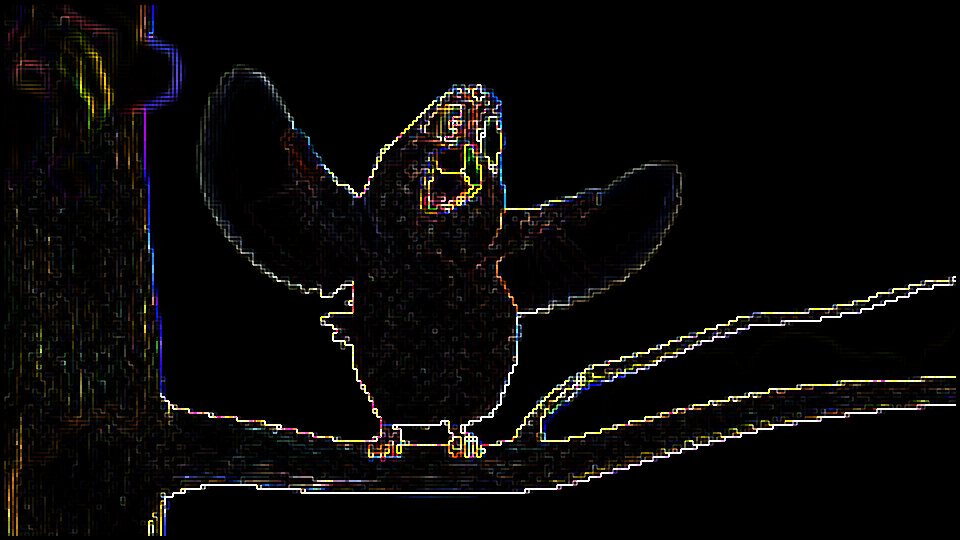
\includegraphics[width=0.3\textwidth]{media/bird-edgetv}
  }
  \subfigure[Filtro ``revtv''.]{
    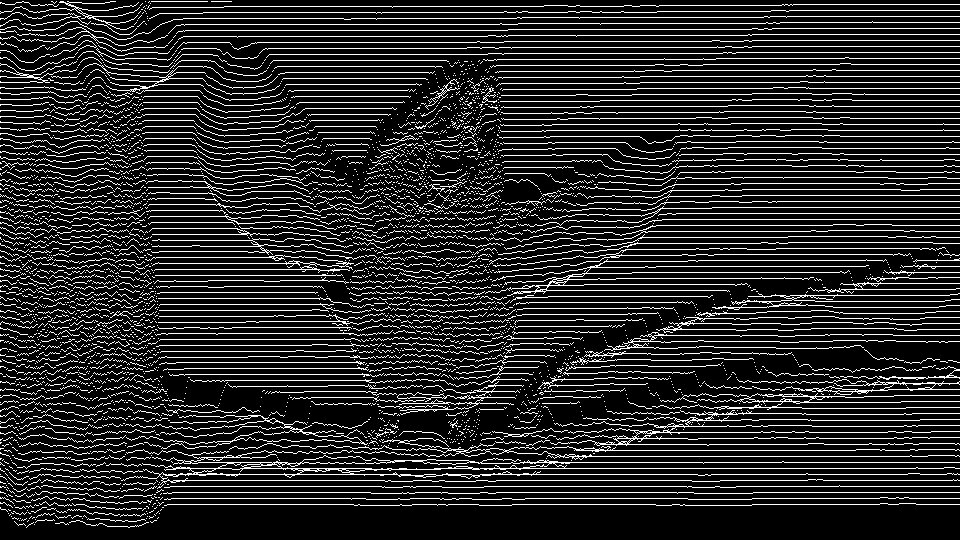
\includegraphics[width=0.3\textwidth]{media/bird-revtv}
  }
  \caption{Efeitos de vídeo aplicados pelo \en{script} da
    Listagem~\ref{lst:filtros-sh}.}
  \label{fig:filtros-screen}
\end{figure*}
\vskip-\baselineskip

Concluindo a seção, a Listagem~\ref{lst:filtros} apresenta um trecho do
programa~C equivalente ao \en{script} da Listagem~\ref{lst:filtros-sh}.
O trecho corresponde ao código da \en{callback} \C{pad_added_cb} disparada
pelo sinal ``pad-added'' do elemento ``uridecodebin''.  O código da função
\C{main} apesar de omitido é trivial.  Ele cria um elemento
``uridecodebin'', atribui à sua propriedade ``uri'' o primeiro argumento do
programa, registra em seu sinal ``pad-added'' a \en{callback}
\C{pad_added_cb} e passa como dado opcional da \en{callback} o segundo
argumento do programa (número entre~0--4 que determina os filtros
selecionados).  Em seguida, a \en{thread} da aplicação transiciona o
\en{pipeline} para \en{playing} e aguarda o fim da reprodução antes de
liberar os dados alocados e terminar o programa.  A operação da
\en{callback} é similar àquela da Listagem~\ref{lst:ogg}.  A diferença aqui
é que os filtros são criados de acordo com o segundo argumento da aplicação
(inteiro passado por referência à \en{callback} via o parâmetro~\C{data}).
\rg{Por que não passar o nome do filtro como parâmetro para a aplicação?
    Tornaria o programa mais genérico.}

\lstinputlisting[
style=display,
firstline=4,
lastline=99,
caption={Trecho do programa~C equivalente ao \en{script}
da Listagem~\ref{lst:filtros-sh}.},
label={lst:filtros},
]{src/filter.c}


\section{Adicionando os controles~\en{play}, \en{pause},
\en{stop}, \en{seek}, \en{fast-foward} e~\en{rewind}}
\label{sec:ops}

Os programas que vimos até agora não são interativos.  Assim que inciados,
eles constroem um \en{pipeline} que reproduz o conteúdo uma única vez, do
inicio ao fim.  Nesta seção vamos adicionar os controles \en{play},
\en{pause}, \en{stop}, \en{seek}, \en{fast-forward} e \en{rewind} ao
programa ``Olá mundo'' da Listagem~\ref{lst:hello}.  Nosso objetivo é fazer
com que o programa responda aos seguintes comandos de tecla:
\begin{center}
  \begin{tabular}{cl}
    \keystroke{SPC} & pausa ou resume a reprodução
                      (\en{pause} e \en{play})\\[2\jot]
    \keystroke{$\to$} & avança~5s (\en{seek})\\[2\jot]
    \keystroke{$\leftarrow$} & retrocede~5s (\en{seek})\\[2\jot]
    \keystroke{F} & reproduz 2x mais rápido (\en{fast-foward})\\[2\jot]
    \keystroke{R} & reproduz ao contrário 2x mais rápido
                    (\en{rewind})\\[2\jot]
    \keystroke{N} & reproduz na velocidade original\\[2\jot]
    \keystroke{Q} & para a reprodução e termina o programa (\en{stop})
  \end{tabular}
\end{center}

Observe que escolhemos o programa ``Olá mundo'' apenas para simplificar as
listagens apresentadas.  Os mecanismos para captura de teclas e controle do
\en{pipeline} descritos sobre esse exemplo são gerais e se aplicam a
qualquer aplicação GStreamer.  Nesse caso, para obter teclas vamos capturar
as mensagens de eventos de navegação (\C{GST_NAVIGATION_MESSAGE_EVENT})
postadas pelo \en{sink} de vídeo no \en{bus} do \en{pipeline}.  Já para
implementar as operações de \en{play}, \en{pause} e \en{stop}, vamos
transicionar o \en{pipeline} para os estados correspondentes.  E para
implementar as operações \en{seek}, \en{fast-foward} e \en{rewind}, vamos
postar eventos de \en{seek} (\C{GST_EVENT_SEEK}) que requisitam mudanças na
posição e na taxa de reprodução do conteúdo.

A Listagem~\ref{lst:controles-main} apresenta o trecho de código contendo a
função \C{main} do novo programa ``Olá mundo'' (versão com controles).  Até
a linha~28, o código da função é idêntico ao código correspondente na
Listagem~\ref{lst:hello}.  A diferença aqui está na forma como capturamos
mensagens postadas no \en{bus}.  Até agora, para obter mensagens do
\en{bus}, usamos função \C{gst_bus_timed_pop_filtered}, que bloqueia a
\en{thread} da aplicação até que tipos específicos de mensagens sejam
postados.  Na Listagem~\ref{lst:controles-main}, como a aplicação é
orientada a eventos, usamos uma técnica diferente, baseada no \en{loop} de
eventos da~GLib (\C{GMainLoop}).

O \en{loop} de eventos é criado pela chamada~\C{g_main_loop_new} na linha~28
da Listagem~\ref{lst:controles-main}.  O primeiro argumento da
chamada~(\C{NULL}) indica que o \en{loop} irá receber eventos de qualquer
fonte registrada via~GLib\footnote{Veja~\cite{glib} para mais informações
  sobre \en{loops} de eventos na GLib.}, e o segundo argumento~(\C{FALSE})
indica que o \en{loop} não deve ser iniciado imediatamente (iniciaremos o
\en{loop} posteriormente na linha~35).

As chamadas \C{g_object_set_data} seguintes (linhas~30--31) armazenam no
\en{bus} ponteiros para o \en{pipeline} e para o \en{loop}.  Observe que o
\en{bus} (\C{GstBus}) também é um objeto (\C{GObject}) e, como todo objeto,
possui uma tabela \en{hash} em que podem ser armazenados dados de usuário
(\en{user~data}).  No caso, a chamada das linhas~30--31 armazenam na
\en{hash} do \en{bus} um ponteiro para o \en{pipeline}, indexado pela chave
``pipeline'', e um ponteiro para o \en{loop}, indexado pelo \en{loop}.  Isso
é necessário porque mais tarde, na \en{callback} do \en{bus}, não temos
acesso direto à esses objetos.

A chamada \C{gst_bus_add_watch} (linha~32) registra a \en{callback}
\C{bus_cb} como tratadora (\en{listener}) de mensagens \en{bus}.  Ou seja, a
\en{callback} será chamada no \en{loop} de eventos sempre que uma mensagem é
postada no \en{bus}.  E a chamada seguinte (linha~33) libera a referência
obtida na linha~28.

A chamada \C{g_main_loop_run} (linha~35) inicia o \en{loop} de eventos da
GLib.  A partir desse ponto a aplicação torna-se orientada a eventos, isto
é, a \en{thread} da aplicação passa a ser controlada pela GLib que apenas
espera eventos e repassa-os às \en{callbacks} registradas (apenas
\C{bus_cb}, no caso).  O controle só volta para a \C{main} quando o \en{loop} é
terminado explicitamente via uma chamada \C{g_main_loop_quit}---o que ocorre
na \en{callback} do \en{bus}.  Nesse caso, as chamadas
restantes~(linhas~37--39) liberam os dados alocados e terminam o programa.

\lstinputlisting[
style=display,
lastline=42,
caption={Função~\texttt{main} do programa ``Olá mundo'' com controles.},
label={lst:controles-main},
]{src/controls.c}

Vejamos agora a operação da \en{callback} \C{bus_cb}, cujo código é apresentado
na Listagem~\ref{lst:controles-cb}.  A cada mensagem postada no \en{bus}, o
\en{loop} de eventos chama essa \en{callback} com os seguintes argumentos: o
\en{bus}, a mensagem postada e o dado adicional passado à função
\C{gst_bus_add_watch} (linha~32 da Listagem~\ref{lst:controles-main}) no
momento do registro da \en{callback} (no caso, \C{NULL}).

Na Listagem~\ref{lst:controles-cb}, as chamadas das linhas~3 e~4 obtém as
referências, respectivamente, para o \en{pipeline} e para o \en{loop}
armazenadas na \en{hash} do \en{bus}.  O comando \C{switch} seguinte
(linhas~5--37) trata a mensagem recebida de acordo com o seu tipo.  Há três
possibilidades:
\begin{enumerate}
\item Se a mensagem indica um erro ou o fim do fluxo (EOS), a \en{callback}
  termina o \en{loop} de eventos (linha~40) e remove a si mesmo da lista de
  tratadores (linha~41).
\item Se a mensagem é uma mensagem de elemento (linha~10), é também mensagem
  de evento de navegação (linhas~14--15) e indica um evento de
  pressionamento de tecla (linhas~18--19), então a \en{callback} executa a
  operação associada à tecla pressionada.\footnote{Além de teclas, as
    mensagens de evento de navegação podem ser usadas para capturar a
    movimentação e cliques de botões do mouse.}  Ou seja, a \en{callback}
  chama a função auxiliar \C{toggle_pause} se a tecla é ``space'', chama a
  função auxiliar \C{seek} se a tecla é ``right'' ou ``left'', chama a
  função auxiliar \C{speed} se a tecla é ``f'', ``r'' ou ``n'', e termina o
  \en{loop} se a tecla é ``q''.
\item Em todos os outros casos, a mensagem é ignorada (linha~38).
\end{enumerate}

\lstinputlisting[
style=display,
firstline=94,
caption={Função~\texttt{bus\_cb} do programa ``Olá mundo'' com controles.},
label={lst:controles-cb},
]{src/controls.c}

A Listagem~\ref{lst:controles-aux} apresenta o código das funções
auxiliares~\C{toggle_pause}, \C{seek} e~\C{resume} chamadas pela
\en{callback} \C{bus_cb} da Listagem~\ref{lst:controles-cb}.

A função~\C{toggle_pause} (linhas~1--12) alterna o estado do \en{pipeline}
entre \en{paused} e \en{playing} dependendo do estado atual:  se o
\en{pipeline} está pausado ela o inicia, e se o \en{pipeline} está tocando
ela o pausa.

A função \C{seek} (linhas~14--23) requisita um salto de \C{offset}
nanosegundos (ns) na reprodução do conteúdo a partir do seu ponto atual.
A chamada da linha~17 obtém o tempo absoluto do \en{pipeline} (ns) e
armazena-o em \C{from}.  A atribuição seguinte calcula o tempo absoluto (ns)
em que o \en{pipeline} deve estar após o salto e armazena em \C{to}.
Finalmente, a chamada \C{gst_element_seek_simple} (linhas~19--22) requisita
o salto para o novo tempo absoluto~\C{to}.  A função
\C{gst_element_seek_simple} recebe quatro argumentos: o elemento alvo da
operação, o formato do deslocamento, \en{flags} opcionais e o valor do
deslocamento.  O formato (segundo argumento) indica o formato em que o
descolocamento está especificado---no caso, usamos \C{GST_FORMAT_TIME} para
indicar um deslocamento no tempo.  As \en{flags} (terceiro argumento)
determinam a característica da operação: a \en{flag}
\C{GST_SEEK_FLAG_ACCURATE} indica que a operação deve ter uma precisão
razoável, a \en{flag} \C{GST_SEEK_FLAG_FLUSH} indica que \en{caches}
internos de elementos subsequentes devem ser descartados e a \en{flag}
\C{GST_SEEK_FLAG_FLUSH} indica que (se possível) durante a operação apenas
quadros chave (\en{key~frames}) devem ser decodificados.

A última função, \C{speed}, (linhas~25--49) requisita uma mudança na taxa de
reprodução do \en{pipeline} de acordo com o parâmetro \en{rate}.  Esse tipo
de mudança de taxa é feita por meio da função \C{gst_element_seek}, que é
também utilizada para realizar operações de \en{seek} complexas.  Essa
função recebe oito argumentos: (1)~o elemento alvo; (2)~a nova taxa de
reprodução; (3)~o formato dos deslocamentos; (4)~\en{flags} opcionais; (5)~o
tipo do início do desolamento; (6)~o novo inicio; (7)~o tipo do fim do
deslocamento; e~(8) o novo fim.  Como aqui nosso objetivo é apenas alterar a
taxa de reprodução o deslocamento é a própria posição atual do \en{fluxo}
(variável \C{from} preenchida na linha~37).  Se a taxa é positiva, o
deslocamento é relativo ao início (linhas~32--38), caso contrário
ele é relativo ao fim (linhas~39--45).  Na pratica, valores de taxa
superiores a~1 aumentam a velocidade de reprodução.  Valores entre~0 e~1
fazem o conteúdo tocar em câmera lenta.  E valores negativos fazem o
conteúdo tocar ao contrário.

\lstinputlisting[
style=display,
firstline=44,
lastline=92,
caption={Funções~\texttt{toggle\_paused}, \texttt{seek} e~\texttt{speed}
do programa ``Olá mundo'' com controles.},
label={lst:controles-aux},
]{src/controls.c}


\section{Plugins}
\label{sec:plugins}
Até agora só vimos como usar elementos já definidos pelo Gstreamer.  Nesta
seção iremos discutir como é possível criar novos tipos de elementos---os quais
podem ser distribuidos separadamente, instalados e usados em um
\emph{pipeline}.  Um plugin no Gstreamer nada mais é do que um tipo de ator (ou
``elemento'') que pode ser instanciado em um pipeline.

%Esta seção apresenta um exemplo e discute a API de plugins do Gstreamer.
%Espera-se que ao final dela, o leitor tenha uma visão geral de como criar novos
%tipos de elementos que podem ser usados em um \emph{pipeline}.

%Os plugins do Gstreamer podem ser divididos em quatro categorias principais:
%\emph{source}, \emph{sink}, \emph{transform}, and \emph{processing} plugin.

Os plugins do Gstreamer são derivados da classe base \emph{GstElement}.  Além
disso, outras classes distribuídas nos pacotes gst-plugin-base também podem ser
usadas para criar novos plugins.  As principais são:

\begin{itemize}
%  \item{GstElement}--a classe base mais genérica, das quais as outras classes
%                     bases derivam;
  \item{GstBaseSrc}--classe base para plugins tipo \emph{source} (ou
                     produtores);
  \item{GstBaseSink}--classe base para plugins do tipo \emph{sink} (ou
                      consumidores);
  \item{GstBaseTransform}--classe base para plugins do tipo \emph{tranform}; e
  \item{GstBin}---cria um manipuladores de plugins customizáveis similar ao
                  GstPipeline.
\end{itemize}

\tikzstyle{every node}=[draw=black,thick,anchor=west]
\tikzstyle{selected}=[draw=red,fill=red!30]
\tikzstyle{optional}=[dashed,fill=gray!50]
\begin{figure}[H]
  \centering
  \begin{tikzpicture}[%
  grow via three points={one child at (0.5,-0.7) and
  two children at (0.5,-0.7) and (0.5,-1.4)},
  edge from parent path={(\tikzparentnode.south) |- (\tikzchildnode.west)}]
  \node {GObject}
    child {
%      node {GInitiallyUnknown}
%      child {
        node {GstElement}
        child {node{GstBaseSrc}}
        child {node{GstBaseSink}}
        child {node{GstBin}}
        child {
          node {GstBaseTransform}
          child {node {GstAudioFilter}}
          child {node {GstVideoFitter}}
        }
%      }
    };
  \end{tikzpicture}
  \label{fig:class_hierarchy}
\end{figure}

\subsection*{Comunicação entre os plugins}
Como mencionado anteriormente, a comunicação entre os elementos é gerenciada
usando \emph{pads}.  Sendo assim, ao criar um plugin também devemos especificar
quantos e quais tipos de \emph{pad} esse plugin aceita como entrada e saída.

%Um \emph{pad} pode ser visto como um conector que conecta dois plugins
%(similar ao cabo de força que conecta uma tomada na parede ao DVD player).

A comunicação entre os plugins pode ser classificada em duas subcategorias:
\emph{mensagens de controle} (ou eventos) e \emph{mensagens de conteúdo de
mídia} (ou buffers).  As mensagens de controle são cruciais para controlar o
processamento das mídias.  As mensagens de conteúdo de mídia são responsáveis
por transferir o conteúdo que precisa ser processado.

\subsection*{Funções}
\begin{itemize}
  \item plugin\_init
  \item chain: Essa função é onde todo o processamento dos dados é realizado.
        No caso de plugins simples as funções \_chain () são geralmente lineares,
        para cada buffer na enntrada um buffer será gerado na saída também.
        Below is a very simple implementation of a chain function: 
  \item event
\end{itemize}

\subsection*{Exemplo de plugin}
Plugin simples contendo 1 sink pad e 1 source pad.

Apenas multiplica o dado de entrada por um número X.

\subsection*{Testando o seu plugin}
Para compilar o nosso plugin devemos gerar uma biblioteca dinâmica (.dll no
Windows ou .so no Linux).  O comando a seguire compila o exemplo desenvolvido
acima:

\begin{lstlisting}[style=command]
@\$@ cc -share -fPIC \
  `pkg-config --cflags --libs gstreamer-1.0 gstreamer-base-1.0`\
  simplefilter.c -o simplefilter.so
\end{lstlisting}

O comando a seguir carrega o plugin myfilter que desenvolvemos em um pipeline
simples:

\begin{lstlisting}[style=command]
@\$@ gst-launch-1.0 --gst-plugin-path=. \
     audiotestsrc ! audioconvert ! myfilter ! alsasink
\end{lstlisting}

\noindent compare com o resultado sem o nosso filtro:
\begin{lstlisting}[style=command]
@\$@ gst-launch-1.0 --gst-plugin-path=. \
     audiotestsrc ! audioconvert ! alsasink
\end{lstlisting}





\section{Conclusão}
\label{sec:conclusao}
Neste minicurso apresentamos uma visão introdutória do \en{framework} GStreamer. 
Discutimos o modelo de \en{dataflow} no qual ele se baseia e como esse modelo
é implementado internamente utilizando os conceitos de elementos, \en{pads} e 
\en{pipeline}. Por meio da implementação de vários exemplos mostramos como
se dá o processo de desenvolvimento de aplicações no GStreamer. No entanto,
como o \en{framework} é bastante abrangente, alguns tópicos avançados não
foram apresentados. Aqui discutimos rapidamente alguns desses tópicos 
para nortear os leitores sobre a existência dessas funcionalidades. 

O GStreamer dá suporte à implementação de aplicações que transmitem e/ou
recebem dados pela rede. Por exemplo, o pacote \en{gst-plugins-good} implementa
vários elementos que podem ser usados para criar servidores de \en{streaming}
RTP/RTCP/RTSP. Em linhas gerais, um servidor RTP deve empacotar fluxos
codificados em um dado formato em pacotes RTP e enviá-los por meio do 
protocolo UDP, como ilustrado no \en{pipeline} da Figura~\ref{fig:rtp-server}.
O elemento \en{rtptheorapay} recebe um fluxo de vídeo Theora e o encapsula
em pacotes RTP que são enviados pela rede pelo elemento \en{udpsink} usando
o protocolo UDP. De forma análoga, um cliente para esse servidor poderia ser 
implementado usando o elemento \en{udpsrc}, que recebe um fluxo de dados UDP,
conectado ao elemento \en{rtptheoradepay}, que desempacota os pacotes RTP gerando
como saída um fluxo de vídeo Theora, como ilustrado no \en{pipeline} da
Figura~\ref{fig:rtp-client}. Além de elementos que encapsulam e desencapsulam 
formatos específicos de fluxos em pacotes RTP, no GStreamer há diversos outros 
elementos que facilitam a implementação de aplicações de \en{streaming}, como
por exemplo \en{rtpmanager}, \en{rtpbin}, \en{rtpjitterbuffer}, etc.

\begin{figure}[H]
  \centering
  \subfigure [Servidor RTP]
  {
    \begin{tikzpicture}
      \node (filesrc) [element] {filesrc};
      \node (oggdemux) [element, right of=filesrc] {oggdemux};
      \node (rtptheorapay) [element, right of=oggdemux] {rtptheorapay};
      \node (udpsink) [element, right of=rtptheorapay] {udpsink};
      \draw [->, arrow] (filesrc) -- (oggdemux);
      \draw [->, arrow] (oggdemux) -- (rtptheorapay);
      \draw [->, arrow] (rtptheorapay) -- (udpsink);
    \end{tikzpicture}
    \label{fig:rtp-server}
  }
  \subfigure [Cliente RTP]
  {
    \begin{tikzpicture}
      \node (udpsrc) [element] {udpsrc};
      \node (rtptheoradepay) [element, right of=udpsrc] {rtptheoradepay};
      \node (theoradec) [element, right of=rtptheoradepay] {theoradec};
      \node (xvimagesink) [element, right of=theoradec] {xvimagesink};
      \draw [->, arrow] (udpsrc) -- (rtptheoradepay);
      \draw [->, arrow] (rtptheoradepay) -- (theoradec);
      \draw [->, arrow] (theoradec) -- (xvimagesink);
    \end{tikzpicture}
    \label{fig:rtp-client}
  }
  \caption{\en{Pipeline}s de um servidor e cliente RTP para vídeos 
    OGG codificados no formato Theora.}
  \label{fig:pipe-rtp-server}
\end{figure}

Internamente, \en{pipelines} mantém um relógio do tipo \C{GstClock} usado
para sincronizar a exibição dos \en{buffers}. Elementos \en{sink} usam esse
relógio para controlar a renderização dos dados, bem como para descartar
\en{buffers} que chegam atrasados. É possível sincronizar o relógio de 
\en{pipelines} diferentes (mesmo em máquinas separadas) por meio dos objetos
\C{GstNetTimeProvider} (expõe o tempo de um \C{GstClock} para a rede) 
e \C{GstNetClientClock} (sincroniza o relógio de um \en{pipeline} a um
objeto provedor de tempo -- \C{GstNetTimeProvider}), por exemplo. É possível
ainda criar relógios sincronizados com um servidor NTP (\C{GstNtpClock}) 
ou PTP (\C{GstPtpClock}).

O GStremaer permite que dados sejam adicionados ou removidos do \en{pipeline}
por meio dos elementos \en{appsrc} e \en{appsink}, respectivamente. \en{Appsrc}
é um elemento do tipo \en{source} e é usado para injetar dados customizados em
um \en{pipeline}. Um típico exemplo de uso desse elemento é na renderização
de um formato de dados não suportado nativamente pelos elementos disponíveis
no GStreamer (essa funcionalidade também pode ser implementada por meio da
criação de um novo elemento, como ilustrado na Seção~\ref{sec:plugins}).
\en{Appsink} é um elemento do tipo \en{sink} usado para receber os \en{buffers}
de saída de uma aplicação. Um cenário de uso para o \en{appsink} é quando se
deseja embutir a saída de um \en{pipeline} em outra uma outra aplicação.

É possível ainda compor diversos vídeos e/ou áudios em um mesmo \en{pipeline}.
Elementos do tipo \en{mix} recebem vários fluxos de um mesmo tipo e geram uma
única saída representando a composição daqueles fluxos. Exemplos de \en{mixers}
de vídeo são os elementos \en{videomix} e \en{compositor}, enquanto os elementos
\en{adder} e \en{audiomixer} são exemplos de \en{mixers} de áudio. 

Um caso de uso alternativo do GStreamer é na transcodificação de mídias. 
É possível criar \en{pipelines} que combinem elementos que decodifiquem
um determinado formato produzindo um fluxo \en{raw} com elementos que recebem
esse fluxo \en{raw} e o codifiquem em outro formato. Nesses casos, o \en{sink}
\en{filesink} pode ser usado para escrever a saída do pipeline em um arquivo.

Este minicurso não tem a pretensão ousada de exaurir todos as funcionalidades
do GStreamer, mas servir como um material introdutório. Consideramos que os 
leitores que tenham conseguido assimilar boa parte dos conceitos aqui
apresentados estejam aptos a se aventurar em outros tópicos mais avançados.
No site oficial do framework~\cite{gstreamer} há diversos materiais (a maioria
em inglês) detalhando o funcionamento interno do GStreamer, bem como alguns
tópicos não abordados aqui. Apesar de não ser essencial, noções do 
\en{framework} GObject ajudam no melhor entendimento do 
funcionamento do GStreamer. Há ainda \en{bindings} do \en{framework} para
outras linguagens\footnote{\url{https://gstreamer.freedesktop.org/bindings/}},
como Python, Java, C++, Qt, Android, Vala, Ruby, Haskell, etc.




\bibliographystyle{plain}
\bibliography{bib}
\end{document}

%  LocalWords:  API start stop fast-forward plugin CLAM ChucK Faust ii iii
%  LocalWords:  bib GStreamer frameworks dataflow player seek rewind Pure
%  LocalWords:  framework DirectShow players fast-foward plugins pads sink
%  LocalWords:  source sources sinks Ogg filesrc oggdemux vorbisdec pad PCM
%  LocalWords:  theoradec alsasink xvimagesink bytes Vorbis Theora raw RGB
%  LocalWords:  demultiplexa-o pulse-code modulation pixels red-green-blue
%  LocalWords:  ALSA CPU QoS quality of service buffers events downstream
%  LocalWords:  upstream EOS end-of-stream flush LocalWords playbin GLib cc
%  LocalWords:  GNOME GObject gst GST init argv bins element factory make
%  LocalWords:  GstElement hello assert nonnull filename bunny ogg Big Buck
%  LocalWords:  Blender Institute Creative Commons object set get free null
%  LocalWords:  string state PLAYING Gstreamer ready paused playing thread
%  LocalWords:  threads streaming bus timed filtered warnings CLOCK NONE cb
%  LocalWords:  MESSAGE msg message unref makefile clean GstObject linker
%  LocalWords:  pkg-config link cflags libs flags glib gstreamer shell all
%  LocalWords:  PROGRAMS LDFLAGS TAB makefiles mad gst-plugins-base LGPL dB
%  LocalWords:  gst-plugins-good Lesser Public License gst-plugins-ugly The
%  LocalWords:  gst-plugins-bad Good the Bad and Ugly coreelements alsa bin
%  LocalWords:  gst-inspect add many GstBin src filter videosink location
%  LocalWords:  main callbacks callback sometimes template caps always user
%  LocalWords:  request pad-added audioconvert queue signal connect added
%  LocalWords:  srcpad demux userdata GstCaps type audio x-vorbis flag has
%  LocalWords:  vorbis video x-theora theora mutexes sinkpad GMutex GCond
%  LocalWords:  gst-launch Bourne equalizer equalizer-nbands bands man band
%  LocalWords:  Properties uridecodebin autovideosink autoaudiosink x-raw
%  LocalWords:  templates transicioná-los basicstyle llll audiofx audioecho
%  LocalWords:  audiodynamic audiopanorama freeverb soundtouch pitch speed
%  LocalWords:  coloreffects effectv shagadelictv dicetv edgetv revtv delay
%  LocalWords:  videocrop videofilter videobalance videoscale script preset
%  LocalWords:  videoconvert intensity room-size level
